\documentclass{patmorin}
\listfiles
\usepackage[utf8]{inputenc}
\usepackage{microtype}
\usepackage{kpfonts}
\usepackage{amsthm,amsmath,amsopn,graphicx}
\usepackage{pat}
\usepackage[letterpaper]{hyperref}
\usepackage[table,dvipsnames]{xcolor}
\usepackage{enumitem}
\definecolor{linkblue}{named}{Blue}
\hypersetup{colorlinks=true, linkcolor=linkblue,  anchorcolor=linkblue,
citecolor=linkblue, filecolor=linkblue, menucolor=linkblue,
urlcolor=linkblue} 
\setlength{\parskip}{1ex}
\usepackage{wasysym}

\DeclareMathOperator*{\argmax}{arg\,max}
\DeclareMathOperator{\cw}{succ}
\DeclareMathOperator{\ccw}{pred}

\title{\MakeUppercase{Notes and Questions on the Expected Performance 
   of Franklin's Leader Election Algorithm}%
   \thanks{This work was partly funded by NSERC and the Ontario Ministry of
    Research, Innovation and Science}}

\author{Probability and Combinatorics 2018}

%\usepackage[mathlines]{lineno}
%\linenumbers
%\setlength{\linenumbersep}{2.5cm}
%\rightlinenumbers
%\linenumbers
%\newcommand*\patchAmsMathEnvironmentForLineno[1]{%
%  \expandafter\let\csname old#1\expandafter\endcsname\csname #1\endcsname
%  \expandafter\let\csname oldend#1\expandafter\endcsname\csname end#1\endcsname
%  \renewenvironment{#1}%
%     {\linenomath\csname old#1\endcsname}%
%     {\csname oldend#1\endcsname\endlinenomath}}% 
%\newcommand*\patchBothAmsMathEnvironmentsForLineno[1]{%
%  \patchAmsMathEnvironmentForLineno{#1}%
%  \patchAmsMathEnvironmentForLineno{#1*}}%
%\AtBeginDocument{%
%\patchBothAmsMathEnvironmentsForLineno{equation}%
%\patchBothAmsMathEnvironmentsForLineno{align}%
%\patchBothAmsMathEnvironmentsForLineno{flalign}%
%\patchBothAmsMathEnvironmentsForLineno{alignat}%
%\patchBothAmsMathEnvironmentsForLineno{gather}%
%\patchBothAmsMathEnvironmentsForLineno{multline}%
%}


\newcommand{\question}[1]{\textbf{\color{red}Question:}~#1}

\DeclareMathOperator{\pw}{pw}

\newcommand{\eps}{\epsilon}



%\pagenumbering{roman}
\begin{document}
%\begin{titlepage}
\maketitle
%
\begin{abstract}
  We present upper and lower-bounds on the performance of an algorithm
  of Franklin for leader election on the ring when the node identifiers
  are independent uniform random variables in $[0,1]$.
\end{abstract}
%\end{titlepage}
%
%\tableofcontents
%
%\newpage


\section{Introduction}
\pagenumbering{arabic}

Franklin's leader election algorithm is a classic algorithm for finding
the maximum value on an $n$-node ring network (a cycle) whose nodes
are have distinct labels $x_0,\ldots,x_{n-1}$ in the order they appear
around the cycle.  The algorithm is initialized with all nodes in an
active state and proceeds in rounds.  During each round, each node
$i$ sends and its label $x_i$ to its nearest active neighbour $i'$ in
the clockwise direction and its nearest active neighbour $i''$ in the
counterclockwise direction.  At the same time node $i$ receives the values
of the labels $x_{i'}$ and $x_{i''}$.  Node $i$ then checks if $x_i <
\max\{x_{i'},x_{i''}\}$ and, if so, node $i$ becomes inactive and does
not partcipate in any subsequent rounds, except to forward messages on
behalf of active nodes.  The algorithm terminates when only one node
remains active.

This algorithm clearly terminates after at most $\log_2 n$ rounds because
at most one out of every two consecutive active nodes remains active after
each round.  If the labels $x_0,\ldots,x_{n-1}$ are independent uniformly
distributed random variables over the interval $[0,1]$, then it seems
plausible that the expected number of rounds in this case is $\log_3 n$.
This seems plausible because, during the first round, node $i$ remains
active if and only if $x_i=\max\{x_{i-1},x_i,x_{i-2}\}$ and this event
clearly has probability $1/3$. Thus, in this probabilistic setting,
the expected number of nodes that remain active after the first round
is $n/3$.

Unfortunately, this argument fails in subsequent rounds because,
after the first round, the labels of active nodes are no longer
independent. Furthermore, a careful calculation (see \secref{p2}) shows
that the probability that a particular node $i$ remains active after 2
rounds approaches
\[
    p_2 = \frac{3e^4 - 48e^2 + 233}{384} \approx 0.1096868681 < 0.111\ldots = 1/9 \enspace .
\]
This is somewhat surprising and suggests that the Franklin leader election algorithm may perform better than expected when identifiers are random.  In particular, it is conceivable that the expected number of rounds in this setting could be $o(\log n)$.


\subsection{The Model and Results}

For a set $S\subseteq\Z$ and any $i\in\Z$, define $\ccw_S(i) =
i-\min\{j\in\N: i-j\in S\}$ and $\cw_S(i) = i+\min\{j\in\N: i+j\in S\}$.
We define $\cw_S^0(i)=\ccw_S^0(i)=i$ and, for $k\in\N$ $\cw_S^k(i) =
\cw_S(\cw_S^{k-1}(i))$ and $\cw_S^{-k}(i) = \ccw_S^{-(k-1)}(i)$.
For a set $S\subseteq\Z$, $\langle X_i: i\in S\rangle$ denotes the
(doubly infinite) sequence in which, for each $i\in S$, the value $X_i$ immediately precedes
the value $X_{\cw_S(i)}$.

To understand Franklin's algorithm as $n\to\infty$, we consider the infinite
case in which the nodes consist of all integers $i\in \Z$ and the labels are
independent uniform random variables $X_i\in[0,1]$, for all $i\in\Z$.

The initial set $A_0$ of active nodes is defined to be $A_0=\Z$ and, at round $r\ge 1$, we determine the set $A_r$ of active nodes after round $r$ as 
\[
    A_r = \{i \in A_{r-1} : X_i = \max\{X_{\ccw_{A_{r-1}}(i)},X_i,
                                      X_{\cw_{A_{r-1}}(i)}\} \} 
\] 
We study the probability $p_r$ that, for some particular $i\in\Z$,
$i\in A_r$.  Intuitively, one would expect that $p_r=1/3^r$, but
we know that this is not even true for $r=2$.  Relaxing this, we might
hope to prove that $\lim_{r\to\infty} p_r^{1/r} = c$ for some $c$ close
to $1/3$.  However, \emph{apriori}, it is not obvious that this limit
exists and, if it does, it may be as large as $1/2$ or as small as $0$.

Here we establish the following upper and lower bounds on $p_r$:

\begin{thm}
   $c_1^r \le p_r \le c_2^r$, where 
   $c_1=0.284519384$ and $c_2= 0.49369977332$.
\end{thm}

We have not been able to establish the existence of the limit
$\lim_{r\to\infty} p_r^{1/r}$ but this result shows that, if
$\lim_{r\to\infty} p_r^{1/r}=c$, then $0 < c_1 \le c\le  c_2 < 1/2$.

In terms of the number of rounds required by Franklin's algorithm on
a finite ring, these results establish that the expected number of
rounds is at most $\log_{1/{c_2}} n + o(\log n)$ and at least $\log_{1/{c_1}}
n- o(\log n)$.  In particular, these results rule out the possibility
that the expected number of rounds is $o(\log n)$.

\section{Derivation of $p_2$}
\seclabel{p2}

Svante's Derivation of $p_2$ can go here.

\section{Tools for Sequences}

The technical difficulty in studying Franklin's algorithm is that, for
$r>1$, the sequence $\langle X_i:i\in A_r\rangle$ is not iid.  In order
to address this difficulty, we study different sets, $L_r\subseteq
A_r\subseteq U_r$ that have the property that the sequences $\langle X_i:i\in
L_r\rangle$ and $\langle X_i:i\in U_r\rangle$ are each independent sets
of random variables, which makes them easier to study. In this way we
obtain upper and lower bounds because
\[
    \Pr\{i\in L_r\} \le \Pr\{i\in A_r\} \le \Pr\{i\in U_r\} \enspace .
\]
To make this work, we need some preliminary results on the structure of
the sequences we are working with.

In the following, all subsets of $\Z$ are infinite and have no maximum
or minimum.  Let $X=\{X_i:i\in \Z\}$ be a set of distinct numbers indexed
by integers.  We say that a subset $S\subseteq\Z$ is \emph{$X$-safe}
if, for every $i\in S$ and
\[
    \max\{X_i,\cw_S(i)\} = \max\{X_m: m\in \{i,\ldots,\cw_S(i)\}\} \enspace .
\]

%See \figref{domination-i}.
%\begin{figure}
%   \begin{center}
%      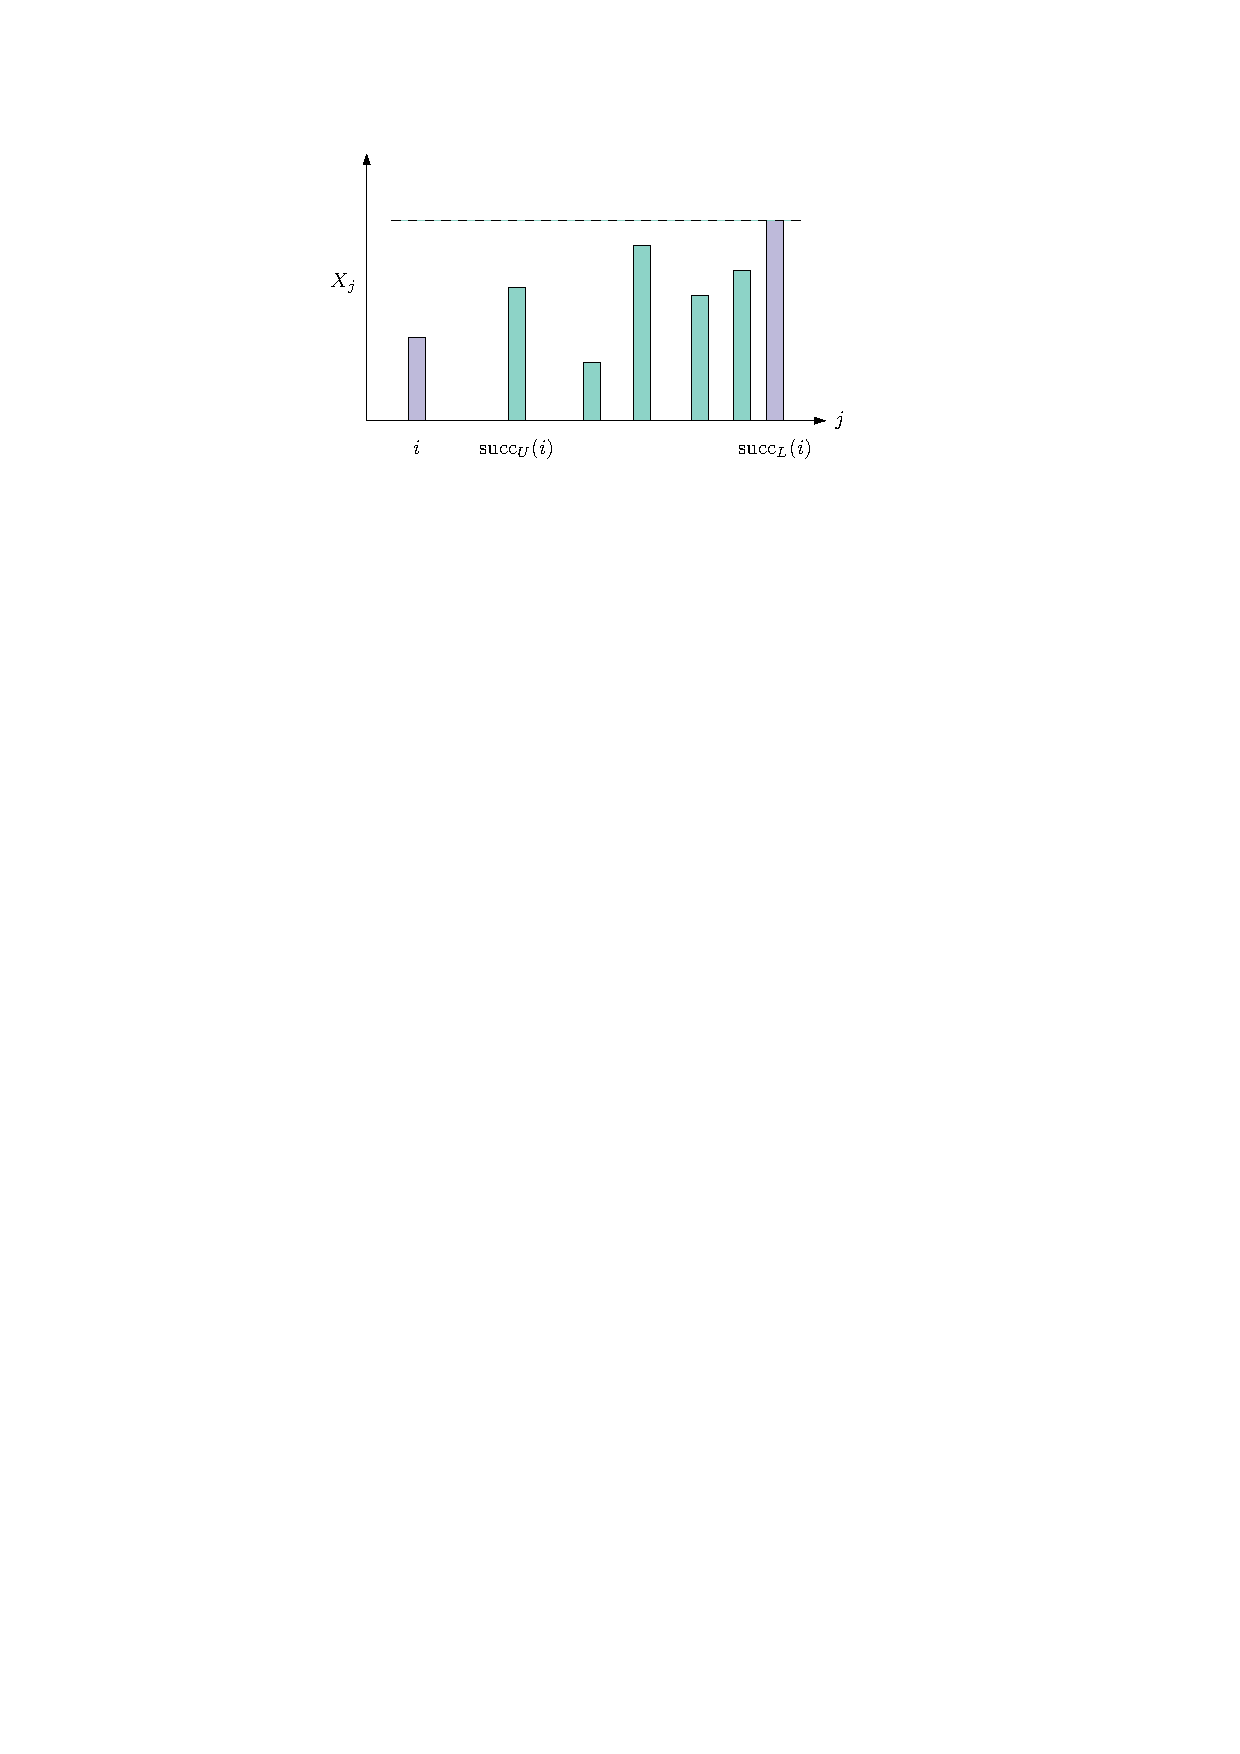
\includegraphics{figs/domination-i}
%   \end{center}
%   \caption{Illustration of \lemref{domination}.}
%   \figlabel{domination-i}
%\end{figure}
%
\begin{lem}\lemlabel{domination}
   Let $L\subseteq U\subseteq\Z$ be sets of integers where $L$
   is $X$-safe.  If $i\in L\cap U$ and $X_{\cw_U(i)} > X_i$, then
   \[
         X_{\cw_L(i)}\ \ge X_{\cw_U(i)} \enspace . 
   \]
   (And the same result holds if we replace all occurrences of $\cw$
   with $\ccw$.)
\end{lem}

\begin{proof}
   Let $j = \cw_U(i)$ and $k=\cw_L(i)$, so $i < j \le k$.
   Since $L\subset U$, $j\in \{i,\ldots,k\}$.  Since $L$ is $X$-safe,
   $\max\{X_i,X_k\} \ge \max\{X_i,\ldots,X_k\} \ge X_j$.  Now we have
   that $\max\{X_i,X_k\} \ge X_j$, but $X_i < X_j$, so it must be that
   $X_k\ge X_j$.
\end{proof}

For any set $A\subset\Z$ and $X=\{X_i:i\in \Z\}$, define the
\emph{Franklin function}
\[
   F(A) = \{ i\in A : X_{i} = \max\{X_{\cw_A(i)},X_i,X_{\ccw_A(i)}\} \}
\]
Notice that for any $r\ge 0$, the set $A_r=F^r_X(\Z)$ is $X$-safe.
With these definitions, the probabilities are are interested in are,
for some fixed $i$, $\Pr\{i\in A_r\}$ for some $r\in\N$.

\section{Lower Bounds}

In this section we prove lower bounds on $p_r$. We begin with a relatively simple argument that shows $p_r \ge 1/4^r$.  

\subsection{A First Attempt: Mountain Peaks}

To prove that $p_r \ge 1/4^r$ we study a
thresholded version of the Franklin function, $F_t$ that produces a
subset of the set $F$ produced by the Franklin function. $F_t$ is a
combination of two kinds of operations: \emph{thresholding} and \emph{max-partitioning}.

\paragraph{Thresholding:}
Let $L\subseteq\Z$ be an $X$-safe set.  Observe that, for any real
value $t$, the \emph{threshold set} $L_{\ge t}=\{i:X_i\ge t\}$ is also an
$X$-safe set. Indeed, for any $i\in L_{\ge t}$, $\max\{X_i,X_{\cw_{L_{\ge t}}(i)}\} = \max\{X_i,\ldots,X_{\cw{L_{\ge t}}(i)}\}$ since $X_i\ge t$, $X_{\cw_{L_{\ge t}}(i)}\ge t$ and $X_{i+1},\ldots,X_{\cw_{L_{\ge t}}(i)-1}$ are all less than $t$.

\paragraph{Max-Partitioning:}
Let $P$ be any partition of $L$ with the property that, for each $I\in
P$, if $i,j,k\in L$ with $i < k$ and $i,k\in I$, then $j\in I$. Then it
is straightforward to verify that the set
\[
     L_{P} = \bigcup_{M\in P} \argmax_{i\in M}(X_i)
\]
is also an $X$-safe set. Indeed, for any $i\in L_{P}$, there exists a $j\in\{i,\ldots,\cw{L_P}(i)-1\}$ such that $X_i=\max\{X_i,\ldots,X_j\}$ and $X_{\cw{L_P}(i)}=\max\{X_{j+1},\ldots,X_{\cw_{L_P}(i)}\}$

\paragraph{Thresholded Franklin:}
Define the graph $G=G(L)$ that has vertex set $L$ and edge set where
$\{(i,\cw_L(i)): i\in L\}$. Remove from $G$ all vertices $i\in L$
such that $X_i < t$ to obtain a graph $G_{\ge t}$ that has a set $P$
of connected components.  We call each connected component of $G_{\ge
t}$ a \emph{mountain}.  Now consider the \emph{$t$-thresholded Franklin
function}
\[
    F_t(L) = \bigcup_{M\in P} \argmax_{i\in V(M)}(X_i) \enspace ,
\]
which keeps the highest \emph{peak} in each mountain.
Note that, for any $t\in\R$, $F_t(L)$ is $X$-safe, since it can be
written as $F_t(L) = (L_{\ge t})_P$.

We will perform a sequence of thresholded Franklin functions
beginning with $\Z$.  For any non-negative integer $r$ and any
real values $t_1,\ldots,t_r$, define $F_{t_1,\ldots,t_r}(L) =
F_{t_r}(F_{t_{r-1}}(\cdots(F_{t_1}(\Z))\cdots ))$.  The following lemma
shows that any such sequence $F_{t_1,\ldots,t_r}(\Z)$ can be used to upper
bound $A_r=F^r(\Z)$

\begin{lem}\lemlabel{lower-domination}
   For any integer $r\ge 0$ and any $t_1,\ldots,t_r$,
   \[  F_{t_1,\ldots,t_r}(\Z) \subseteq F^{r}(\Z)   \]
\end{lem}

\begin{proof}
   Suppose that this is not the case, so that there is some
   minimum value of $r$ and $t_1,\ldots,t_r$ that provides a
   counterexample.  For $m\in\{1,\ldots,r\}$, let $A_m=F^{m}(\Z)$ and let
   $L_m=F_{t_1,\ldots,t_m}(\Z)$.  Since $r$ is minimum, $L_{r-1}\subseteq
   A_{r-1}$ and yet there is some $i\in L_r$ that such that $i\not\in
   A_r$.

   The fact that $i\not\in A_r$ implies that $X_i
   < \max\{X_{\cw_{A_{r-1}}(i)},X_{\ccw_{A_{r-1}}(i)}\}$.
   Suppose, without loss of generality, that $X_i < X_{\cw_{A_{r-1}}(i)}$.
   Now, since $i\in L_r$, it must be that $X_i
   \ge X_{\cw{L_{r-1}}(i)}$.  But, since $L_{r-1}$ is
   $X$-safe, this contradicts \lemref{domination} and the assumption that
   $L_{r-1}\subseteq A_{r-1}$.
\end{proof}

Now that we have established that $F^r(\Z)$ contains $F_{t_1,\ldots,t_r
}(\Z)$, we argue that it is much easier to study the sequence $\langle
X_i:i\in F_{t_1,\ldots,t_r}(\Z)\rangle$ than the sequence $\langle X_i:
i\in F^r(\Z)\rangle$.

\begin{lem}\lemlabel{lower-iid}
   Let $L$ be an $X$-safe set such that $\langle X_i:i\in L\rangle$ is iid.  Then, for any $t$, the sequence $\langle X_i: i\in F_t(L)\rangle$ is iid.
\end{lem}

\begin{proof}
  If $\mathcal{D}$ is the distribution of $X_i$ for each $i\in
  L$ and $p=\Pr\{X_i\ge t\}$, then each $X_j$ with $j\in F_t(L)$
  is distributed like $\max\{Z_1,\ldots,Z_R\}$ where where $R$ is a
  $\mathrm{geometric}(p)$ random variable and each $Z_i$ is an independent
  random variable with distribution $\mathcal{D}$.
\end{proof}

To describe our sequence of subsets $(L_r: r\in\N)$, all that remains
is to describe the sequence of threshold values $(t_r:r\in\N)$ that is
used to obtain each set $L_r = F_{t_1,\ldots,t_r}(\Z)$.  Define the
set $L_0=\Z$.  By assumption, we know that $\langle X_i:i\in L_0\rangle$ is iud
over $[0,1]$.  For $r\ge 1$, \lemref{lower-iid} implies that $\langle X_i:i\in
L_{r-1}\rangle$ is iid over some distribution $\mathcal{D}_{r-1}$ and we take
$t_r$ to be the median of $\mathcal{D}_{r-1}$ so that, for $i\in L_{r-1}$,
$\Pr\{X_i > t_r\}=\Pr\{X_i < t_r\} = 1/2$.

\begin{lem}\lemlabel{lower-bound}
   For any $i\in\Z$ and any $r\in\N$, $\Pr\{i\in L_r\} = 1/4^r$.
\end{lem}

\begin{proof}
   It suffices to prove that $\Pr\{i\in L_r \mid i\in L_{r-1}\} = 1/4$
   since \[ \Pr\{i\in L_r\} = \prod_{k=1}^r \Pr\{i\in L_k\mid i\in L_{k-1}\} .\]

   Perform a relabelling of indices so that, for all $j\in\Z$,
   $Y_j=\cw^j_{L_{r-1}}(i)$. Consider the graph $G_{\ge t}$ described
   above and define the random variable $M_0$ as follows:  If no component
   of $G_{\ge t}$ contains $i$ (because $X_i=Y_0<t_r$) then define $M_0=0$.
   Otherwise, let $C_0$ be the component of $G'$ that contains $i$
   and let $M_0$ be the number of vertices in $C_0$.

   First note that $\Pr\{M_0=0\}=\Pr\{X_i<t_r\}=1/2$.
   For $m \in \N$, 
   \[
       \Pr\{M_0=m\} = m/2^{m+2}
   \]
   since $M_0=m$ precisely if there exists a $k\in\{0,\ldots,m-1\}$
   such that $Y_{-k-1}< t_r$, $Y_{-k+i}<t_r$ and $Y_j \ge t_r$ for all
   $j\in\{-k,\ldots,-k+m-1\}$.  Now we have,
   \begin{align*}
      \Pr\{i\in L_r\mid i\in L_{r-1}\} 
          & = \Pr\{\mbox{$M_0>0$ and $X_i=\max\{X_j:j\in C_0\}$}\} \\
          & = \sum_{m=1}^\infty \Pr\{X_i=\max\{X_j:j\in C_0\}\mid M_0=m\}\Pr\{M_0=m\} \\ 
          & = \sum_{m=1}^\infty (1/i)\Pr\{M_0=m\} \\
          & = \sum_{m=1}^\infty 1/2^{m+2} \\
          & = 1/4 \enspace . \qedhere
   \end{align*}
\end{proof}


Now, by \lemref{lower-domination} and \lemref{lower-bound}, $p_r=\Pr\{i\in
A_r\} \ge \Pr\{i\in L_r\}=1/4$ and we immediately obtain our lower bound:
\begin{cor}
   $p_r \ge 1/4^r$.
\end{cor}


\subsection{A Sharper Lower Bound: Dredging the Lakes}

Next we derive a sharper lower bound using refinements of ideas
from the previous section.

Let $L$ be an $X$-safe set such that $\langle X_i: i\in L\rangle$ is iid
where each element has distribution $\mathcal{D}$.  Again, let $G=(L,E)$
be the graph with vertex set $L$ and edge set $E=\{(i,\cw_L(i)): i\in
L\}$.  Fix a value $0<p<1$ and let $t=t(\mathcal{D},p)$ be chosen so that,
for each $i\in L$, $\Pr\{X_i\ge t\} = p$.  Consider the graph $G_{\ge
t}$ of $G$ induced the elements in $L_{\ge t}$ and consider the subgraph
$G_{<t}$ of $G$ induced by the elements in $L\setminus L_{\ge t}$.

We call the components of $G_{<t}$ \emph{lakes}.  Each lake $C$ of
$G_{<t}$ is a path $v_1,\ldots,v_k$.  For each such lake, we take the set
\[ 
    \hat{C}_t=\{v_j : j\in\{2,\ldots,k-1\},\, X_{v_j}=\max\{X_{v_{j-1}},X_{v_j},X_{v_{j+1}}\}\} \enspace .
\]
That is, $\hat{C}_t$ are the indices of the internal local maxima,
called \emph{seamounts} in the sequence $X_{v_1},\ldots,X_{v_k}$.
Let $\hat{F}_t(L)$ be the union of $\hat{C}_t$ over all components $C$
in $G_{<t}$.

Let $Q_t(L)= F_t(L)\cup \hat{F}_t(L)$. It is straightforward to verify
that $Q_t(L)$ is $X$-safe.  As with $F_t$ define $Q_{t_1,\ldots,t_r}=
Q_{t_k}(\cdots(Q_{t_1}(L))\cdots)$.  The same type of argument used to prove
\lemref{lower-domination} establishes the following result.

\begin{lem}\lemlabel{lower-domination-ii}
   For any integer $r\ge 0$ and any $t_1,\ldots,t_r$,
   \[  Q_{t_1,\ldots,t_r}(\Z) \subseteq F^{r}(\Z)   \]
\end{lem}

To continue the line of reasoning in the previous section, we would like
to prove that the sequence $\langle X_i: i\in Q_t(L)\rangle$ is iid.
Unfortunately, it is not.  Each mountain produces exactly one peak
(in $F_t(L)$), while each lake may produce zero or more seamounts.
The result is that seamounts tend to cluster together.

In what follows, it is helpful to keep this lake/mountain view in
mind. Between every two consecutive mountain peaks (elements of $F_t(L)$)
there is exactly one lake which may or may not contain one or more
seamounts (elements of $\hat{F}_t(L)$.  The following lemma quantifies
the probability that a mountain peak ($i\in F_t(L)$) is immediately
followed by another mountain peak $\cw_{Q_t(L)}(i)$.

\begin{lem}\lemlabel{empty-lake}
  Let $0<p<1$ and select $t$ so that $\Pr\{X_i\ge t\}=p$.  Then,
  for any $i\in F_t(L)$, 
  \[
    \Pr\{\cw_{Q_t(L)}(i) = \cw_{F_t(L)}(i)\} =  
      1-\sum_{m=3}^\infty (1-p)^{m-1}p\left(1-\frac{2^{m-1}}{m!}\right)
  \]
\end{lem}

\begin{proof}
   The event $\cw_{Q_t(L)}(i) = \cw_{F_t(L)}(i)$ occurs precisely
   when $\hat{F}_t(L)$ contains no elements in the interval
   $[i,\cw_{F_t(L)}(i)]$.  We know that there is exactly one lake in
   this interval $C$ in this interval.  Let $C$'s vertices be vertices
   $v_1,\ldots,v_m$ such that $i<v_1<\cdots<v_m<\cw_{F_t(L)}(i)$. The
   lake $C$ does not contribute any element to $\hat{F}_t(L)$ if and
   only if the sequence $X_{v_1},\ldots,X_{v_m}$ has no local maxima
   except possibly $X_{v_1}$ and $X_{v_m}$.

   Since $X_{v_1},\ldots,X_{v_m}$ is iid, the probability that it contains
   no local maxima is equal to the number of permutations with no local
   maxima divided by $m!$.  A straightforward counting argument using
   the binomial identity $\sum_{k=0}^{m-1}\binom{m-1}{k}=2^{m-1}$ shows
   that the number of permutations with no local maxima is $2^{m-1}$
   (see OEIS entry A059204 and references therein \cite{X}).

   Now, the size of the lake $C$ (i.e., the value of $m$) has a
   geometric distribution given by $\Pr\{|C|=m\}=(1-p)^{m-1}p$.
   Letting $\mathcal{E}_C$ denote the event ``$C$  contributes at least
   one elements to $\hat{F}_t(L)$'', we have
   \[
     \Pr\{\mathcal{E}_C\} 
        = \sum_{m=3}^\infty \Pr\{|C|=m\}\Pr\{\mathcal{E}_C\mid |C|=m\} 
        = \sum_{m=3}^\infty (1-p)^{m-1}p\left(1-\frac{2^{m-1}}{m!}\right) 
           \enspace . \qedhere
   \]
\end{proof}

Note that, using the identity $\sum_{k=0}^\infty a^k/(k!)=e^a-1$, one
can derive a closed form for the probability, $q$, in \lemref{empty-lake}:
\[
q = 
1-\frac{p e^{2(1-p)} + p - 2}{2 \, {\left(p - 1\right)}}
\]
(See the accompanying Sage workbook.)

\begin{lem}\lemlabel{lower-bound-ii}
  Let $t$ be chosen as in \lemref{empty-lake}. For any $i\in L$,
  \[ 
       \Pr\{i\in F_t(Q_t(L))\}= (1/2)(2p-p^{2}(1+e^{2-2p}))
  \]
  and the sequence 
  $\langle X_i:i\in F_t(Q_t(L))\rangle$ is iid.
\end{lem}

\begin{proof}
  First note that $i\in F_t(L)$ is a necessary condition for $i\in F_t(Q_t(L))$.
  Mimicing the calculation in the proof of \lemref{lower-bound}, we
  find that, for any $i\in L$, $\Pr\{i\in F_t(L)\}=p-p^2$.

  Let $L'=Q_t(L)$.  Now, for any integer $j$ we have 
  \[
    \Pr\{X_{\cw_{L'}(j)} \ge t\mid j\in F_t(L)\} = 
    \Pr\{\cw_{L'}(j)\in F_t(L)\} = q \enspace .
  \]
  Let $G=G(L')$, condition on $i\in F_t(L)$ and observe that $i$ is part of a mountain $M$ in $L'$.  This mountain has size $a+1+b$ where $a$ counts the number of elements smaller than $i$ and $b$ counts the number of elements greater than $i$.  The distribution of the size of this mountain is given by
  \[
     \Pr\{|M|=m\mid i\in F_t(L)\}\sum_{a=0}^{m-1} q^{a}(1-q)q^b(1-q) = m q^{m-1}(1-q)^2 \enspace .
  \]
  Now, conditional on $i\in F_t(L)$, $i\in F_t(Q_t(L))$ if and only if $i=\max\{X_j: j\in V(M)\}$. The sequence $\langle X_j: j\in V(M)\rangle$ is iid because is a contiguous subsequence of $\langle X_j:j\in F_t(L)\rangle$, which is iid by \lemref{iid}.  In particular, this implies that 
  \[
    \Pr\{i=\max\{X_j: j\in V(M)\}\mid |M|=m \} = 1/m \enspace .
  \]
  Putting everything together, we obtain
  \begin{align*}
    \Pr\{i \in F_t(Q_t(L))\} 
       & = \Pr\{i\in F_t(L)\}\cdot \Pr\{i\in F_t(Q_t(L))\mid i \in F_t(L)\} \\
       & = (p-p^2)\sum_{m=1}^\infty (1/m)\Pr\{|M|=m\mid \mid i \in F_t(L)\} \\
       & = (p-p^2)\sum_{m=1}^\infty q^{m-1}(1-q)^2 \\
       & = (p-p^2)\sum_{m=1}^\infty q^{m-1}(1-q)^2 \\
       & = (p-p^2)(1-q) \\ 
       & = \frac{1}{2} \left(2p-p^{2}(1+e^{2-2p}) \right) \enspace .
  \end{align*}

  To see that $\langle X_i:i\in F_t(Q_t(L))\rangle$ is iid, observe
  that we can obtain an identically distributed sequence by selecting,
  for each $i$, a $\operatorname{geometric}(q)$ random variable $m$
  and setting $X_i=\max\{Z_1,\ldots,Z_m\}$ where $Z_1,\ldots,Z_m$ are
  iid and distributed like the the elements of $\{X_j:j\in F_t(L)\}$.
\end{proof}

Optimizing over $p$, we find that the probability in
\lemref{lower-bound-ii} has a global maximum at $p=-(1/2)W(-2/e^2)$,
where $W$ is the Lambert $W$-function\footnote{$W(z)=x$ where $x$ is
the unique solution to $xe^x = z$.} For this value of $p$,
\[
c_1 = -{\left(e^{{W}(-2/e^2) + 2} + 1\right)} {W}(-2/e^2)^{2}/8 - {W}(-2/e^2)/2
>
0.0809512797364893
\]

\begin{thm}
   For any $k\in\N$, $p_{k} \ge c_1^{k/2} > 0.284519384^k$.
\end{thm}

\begin{proof}
  For even $k$, this follows immediately from $k/2$ applications of
  \lemref{lower-bound-ii}. For odd $k$, it follows $\lfloor k/2\rfloor$
  applications of \lemref{lower-bound-ii} followed by the trivial bound on
  the resulting iid sequence, which shows that $p_{k}\ge c_1^{(k-1)/2}/3
  > c_1^{k/2}$.
\end{proof}

%\begin{lem}\lemlabel{magic}
%   Let $p=5/2-\sqrt{21/4}$, let $t^*$ be chosen so that $\Pr\{X\ge t^*\}=p$, 
%   and let
%   \[  c^*=4\sqrt{21}-18\approx0.330302779823 \enspace . \]
%   Then, 
%   \[  \Pr\{i\in Q_{t^*}(L)\} = c^* = 2\Pr\{i\in F_{t^*}(L)\}=2\Pr\{i\in \hat{F}_{t^*}(L)\} \enspace .
%   \]
%\end{lem}
%
%\begin{proof}
%  First note that $\Pr\{i\in Q_t(L)\}=\Pr\{i\in F_t(L)\} + \Pr\{i\in
%  \hat{F}_t(L)\}$, so it suffices to show that $\Pr\{i\in F_t(L)\} =
%  \Pr\{i\in \hat{F}_t(L)\}=c^*/2$.  Repeating the calculation in the
%  proof of \lemref{lower-bound}, we find that
%  \[
%      \Pr\{i\in F_{t^*}(L)\} = \sum_{m=1}^\infty p^m (1-p)^2 = p-p^2 = 2\sqrt{21}/9 \enspace .
%  \]
%  The calculation for $\hat{F}_{t*}$ is similar except that now, if $i$
%  appears in a component $C$ of $G_{<t^*}$ of size $m\ge 3$, it has
%  probability $(m-2)/3$ of taking part in $\hat{C}_{t^*}$.  This yields
%  \[
%     \Pr\{i\in \hat{F}_{t^*}(L)\} = \sum_{m=3}^\infty (1-p)^mp^2(m-2)/3
%     = -p^3/3 + p^2 - p + 1/3 = 2\sqrt{21}/9 \enspace . \qedhere
%  \]
%\end{proof}
%
%
%\begin{lem}
%   Let $p$, $t^*$, and $c^*$ be defined as in \lemref{magic}.  Then,
%   for any $i\in L$, $\Pr\{i\in F_{t^*}(G_{t^*}(L))\} = c^*/4$ and the
%   sequence $\langle X_i:i\in F_{t^*}(G_{t^*}(L))\rangle$ is iid.
%\end{lem}
%
%\begin{proof}
%   By \lemref{magic} we know that $\Pr\{i\in G_{t^*}(L)\}=c^*$. Let
%   $\mathcal{D}$ be the distribution of $X_i$ conditioned on $i$ being
%   in $G_{t^*}(L)$.  Again, by \lemref{magic} we see that $t^*$ is the
%   median of $\mathcal{D}$.  To be continued....
%\end{proof}
%
%
%\begin{thm}
%   $p_r\ge a^r$ for $a=\sqrt{\sqrt{21}-9/2}\approx 0.287359870121$
%\end{thm}
%



\section{The Upper Bound}

In this section, we prove a modest upper bound, which shows that $p_k <
c_2^k$ for some $c_2\approx 0.479966765528$. 

For an integer set $S\subseteq\Z$ a \emph{blocking} of $S$ is a partition
$B$ of $S$ into ordered sets of sizes 1 and 2, called \emph{blocks},
with the property that, if $(i,i')\in B$, then $i'=\cw_S(i)$.  Note that
this implies that there is a natural total order $\prec_B$ on the
blocks of a blocking $I\prec_B J$ if and only if $\max(I)<\min(J)$.

For a blocking, $B$, of $S$ and a block $I\in B$, we use the notation
$\cw_B(I)=\min\{J\in B: I \prec_B J\}$ where the minimum is defined with
respect to the order $\prec_B$.  The sequence $\langle I: I\in B\rangle$ is the (doubly-infinite) sequence in which, for all $I\in B$, $I$ immediately precedes $\cw_B(I)$.

We define a function $R$ that takes a blocking $B$ of $S$ and produces
another blocking $R(B)$.  Let $B_0$ be the block of $B$ that contains
$\min\{S\cap \N\}$. We partition $B$ into groups of consecutive blocks
in a greedy fashion as follows:  We consider the Starting with a group
$G_0$ that contains $B_0$ we repeatedly add the \ldots Observe that, if the
sequence $\langle I:I\in B\rangle$ of blocks is iid, then the resulting
sequence of groups is iid.

Now, each group contains two or three blocks which contain a total
of three or four integers.  For each such group containing integers
$i_1,\ldots,i_z$, the function $R(B)$ includes exactly one block
that contains only the indices of the one or two local maxima in
$X_{i_1},\ldots,X_{i_z}$.  Note that, since the sequence of groups is iid
and the block output for a group depends only the contents of the group,
the resulting sequence of blocks $\langle I: I\in R(B)\rangle$ is iid.

We are interested in the fraction of the integers in $\cup B$
that make it into $R(B)$.  Let $q_i$, for $i\in\{1,2\}$, denote the
probability that a block in $R(B)$ contains $i$ integers and let $p_{i}$,
$i\in\{3,4\}$ denote the probability that a group in $B$ contains $i$
integers. The quantity of interest is
\[
    \alpha = \frac{q_1+2q_2}{3p_3 + 4p_4} \enspace .
\]
The numerator in this expression represents the ``size'' of $R(B)$
while the denominator represents the ``size'' of $B$.

In a blocking $B$, we classify blocks into three types:
\begin{enumerate}[label=$\alph*$:]
\item \emph{increasing blocks} $(i,i')$ in which $X_{i'} > X_{i}$; 
\item \emph{decreasing blocks} $(i,i')$ in which $X_{i'} < X_{i}$; and
\item \emph{singleton blocks} $(i)$ of size 1.
\end{enumerate}

\begin{figure}
  \begin{center}
  \begin{tabular}{c@{\hspace{.6cm}}c@{\hspace{.6cm}}c@{\hspace{.6cm}}c@{\hspace{.6cm}}c}
     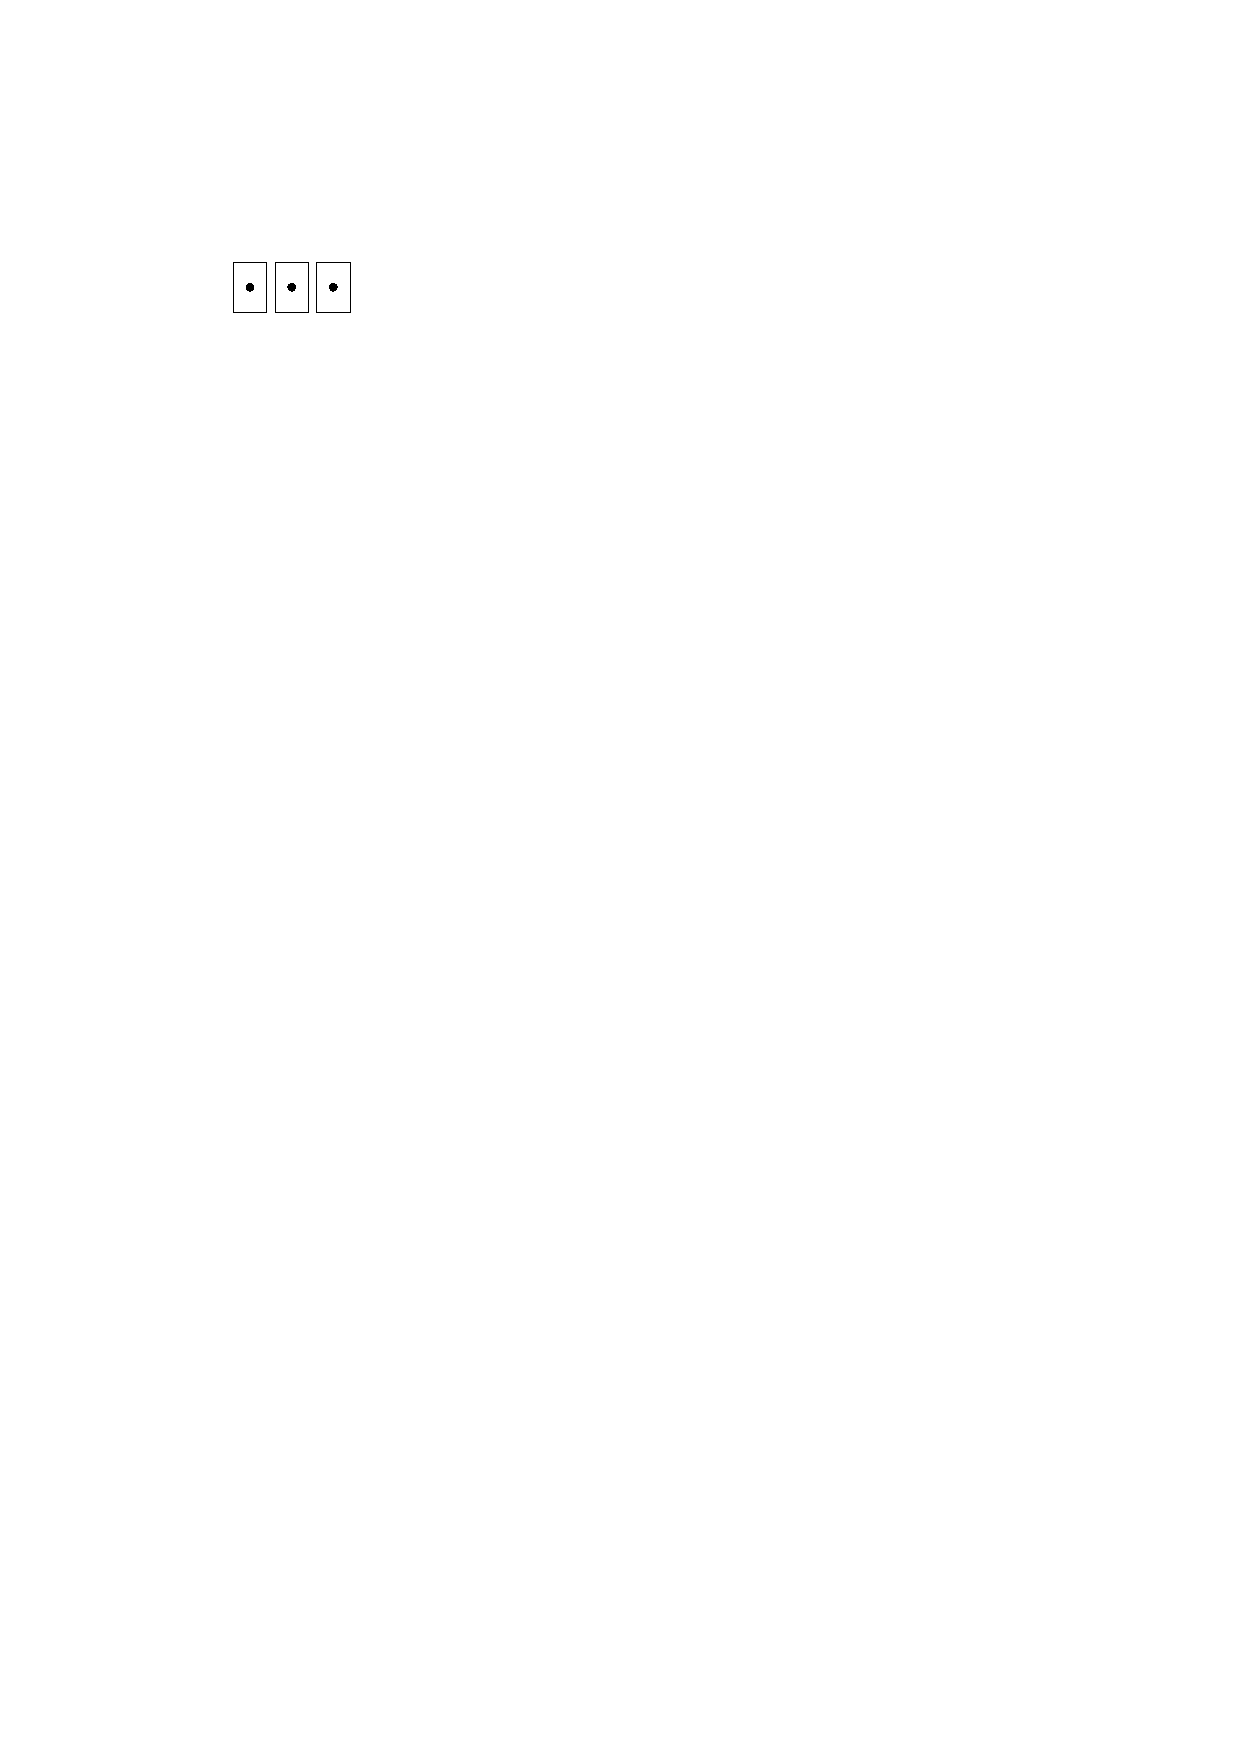
\includegraphics[scale=.625]{figs/c3} &
     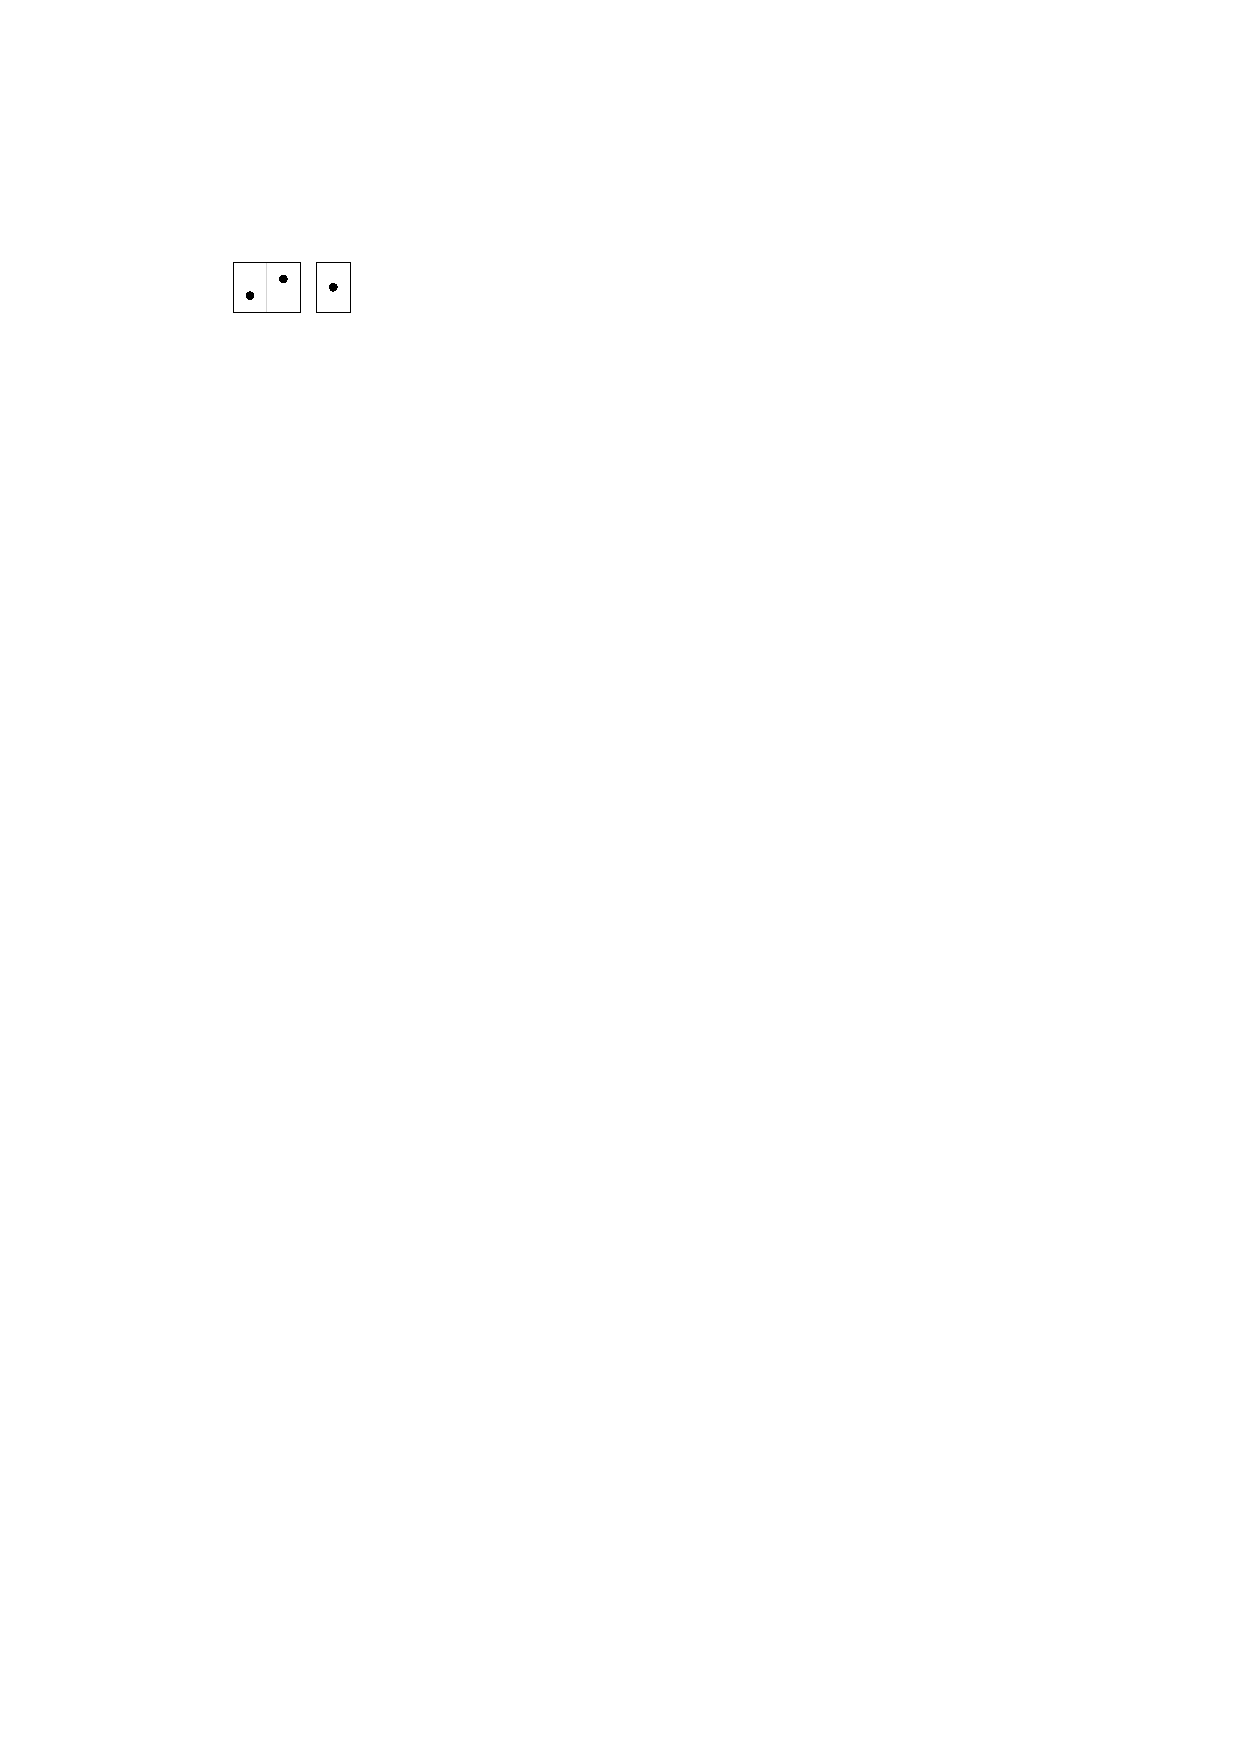
\includegraphics[scale=.625]{figs/ac} &
     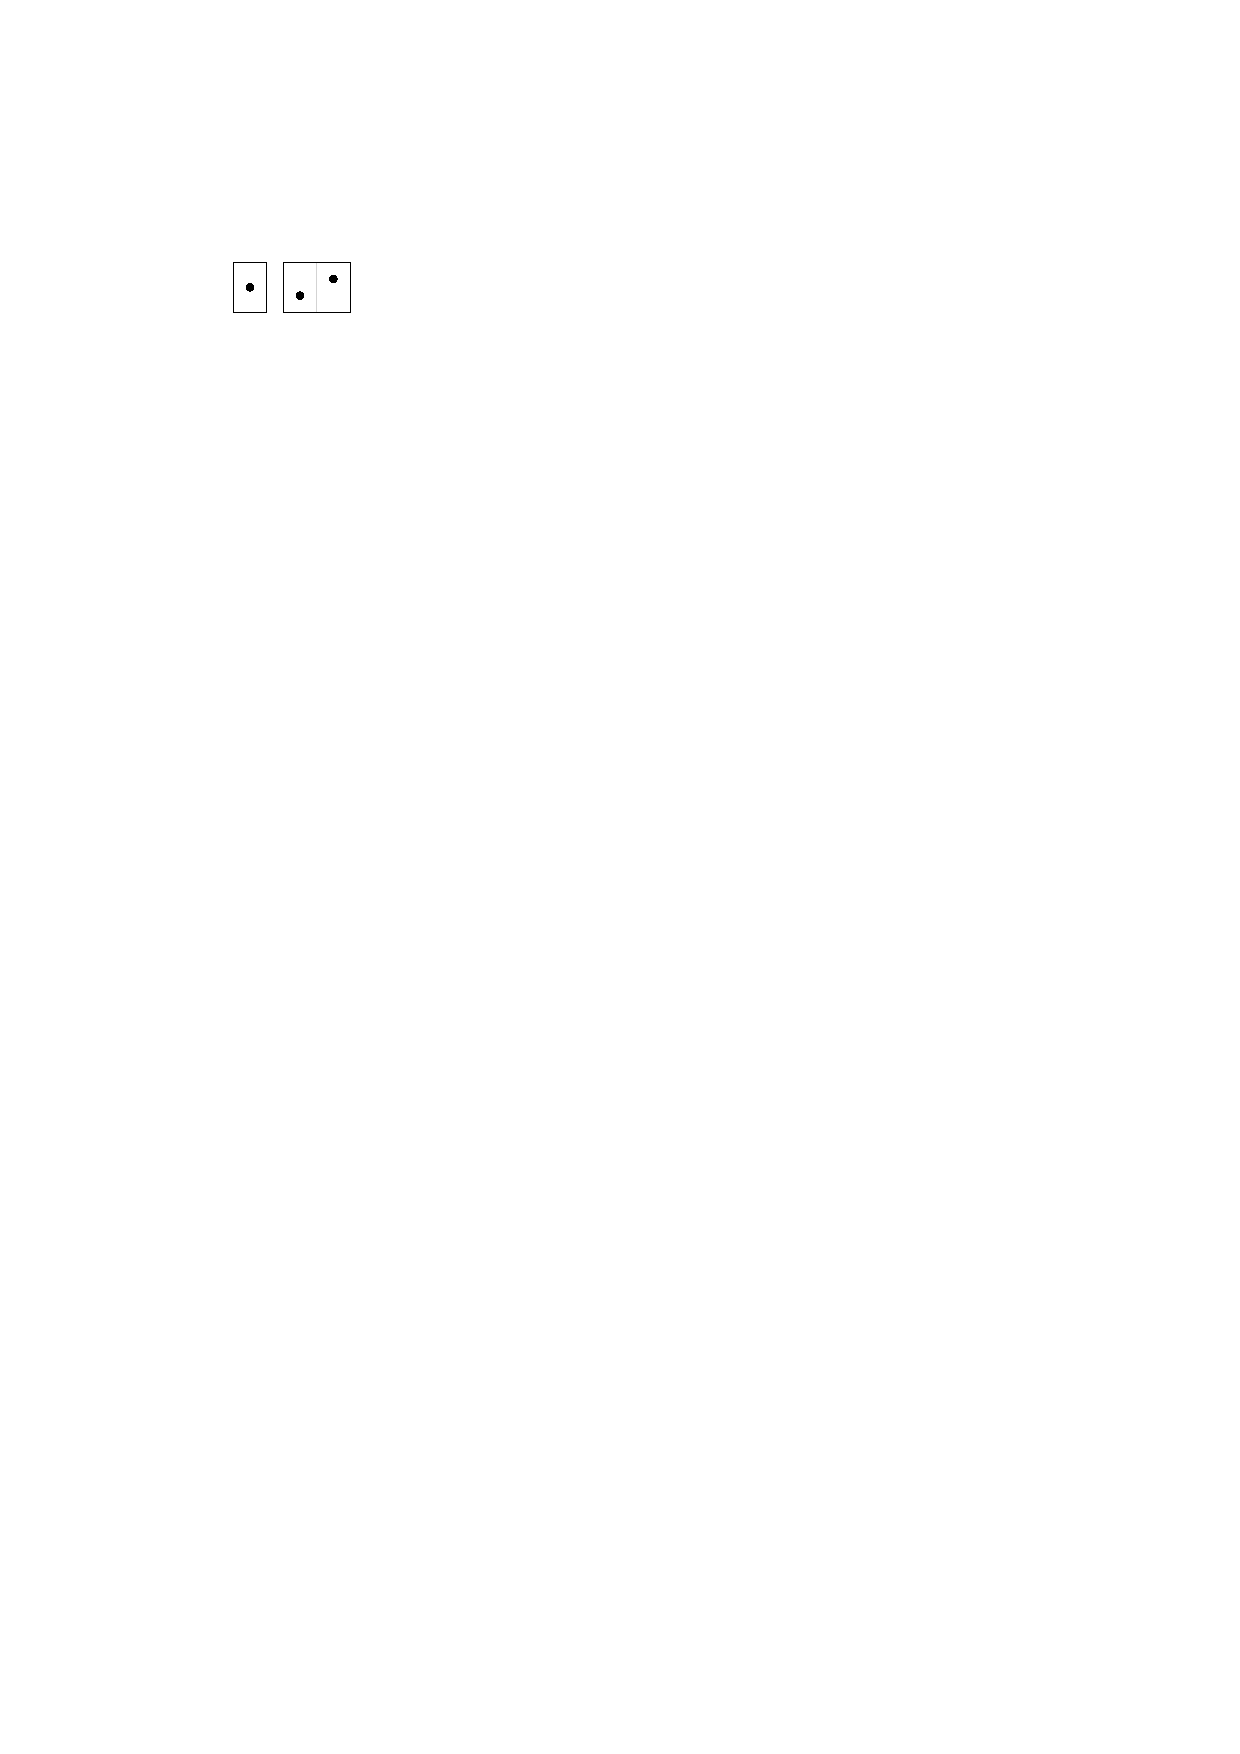
\includegraphics[scale=.625]{figs/ca} &
     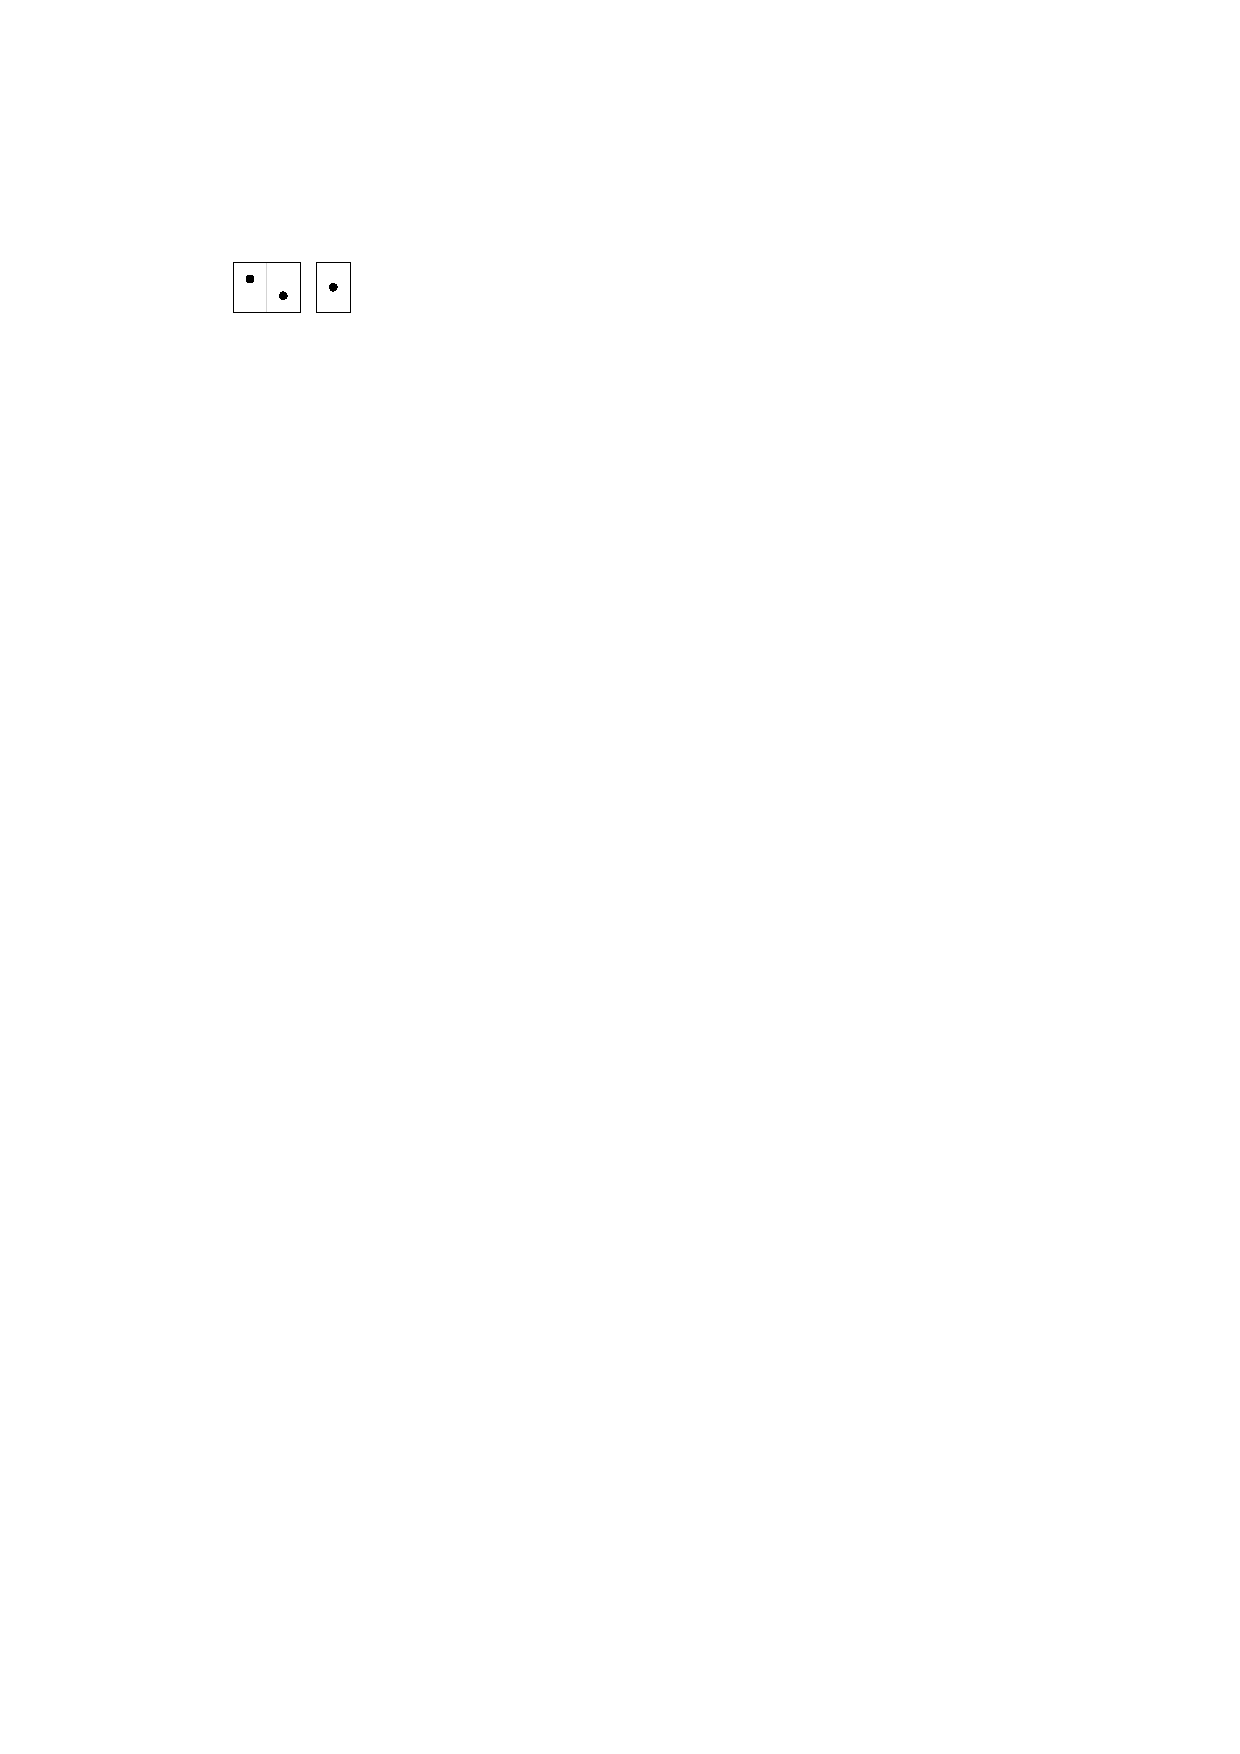
\includegraphics[scale=.625]{figs/bc} &
     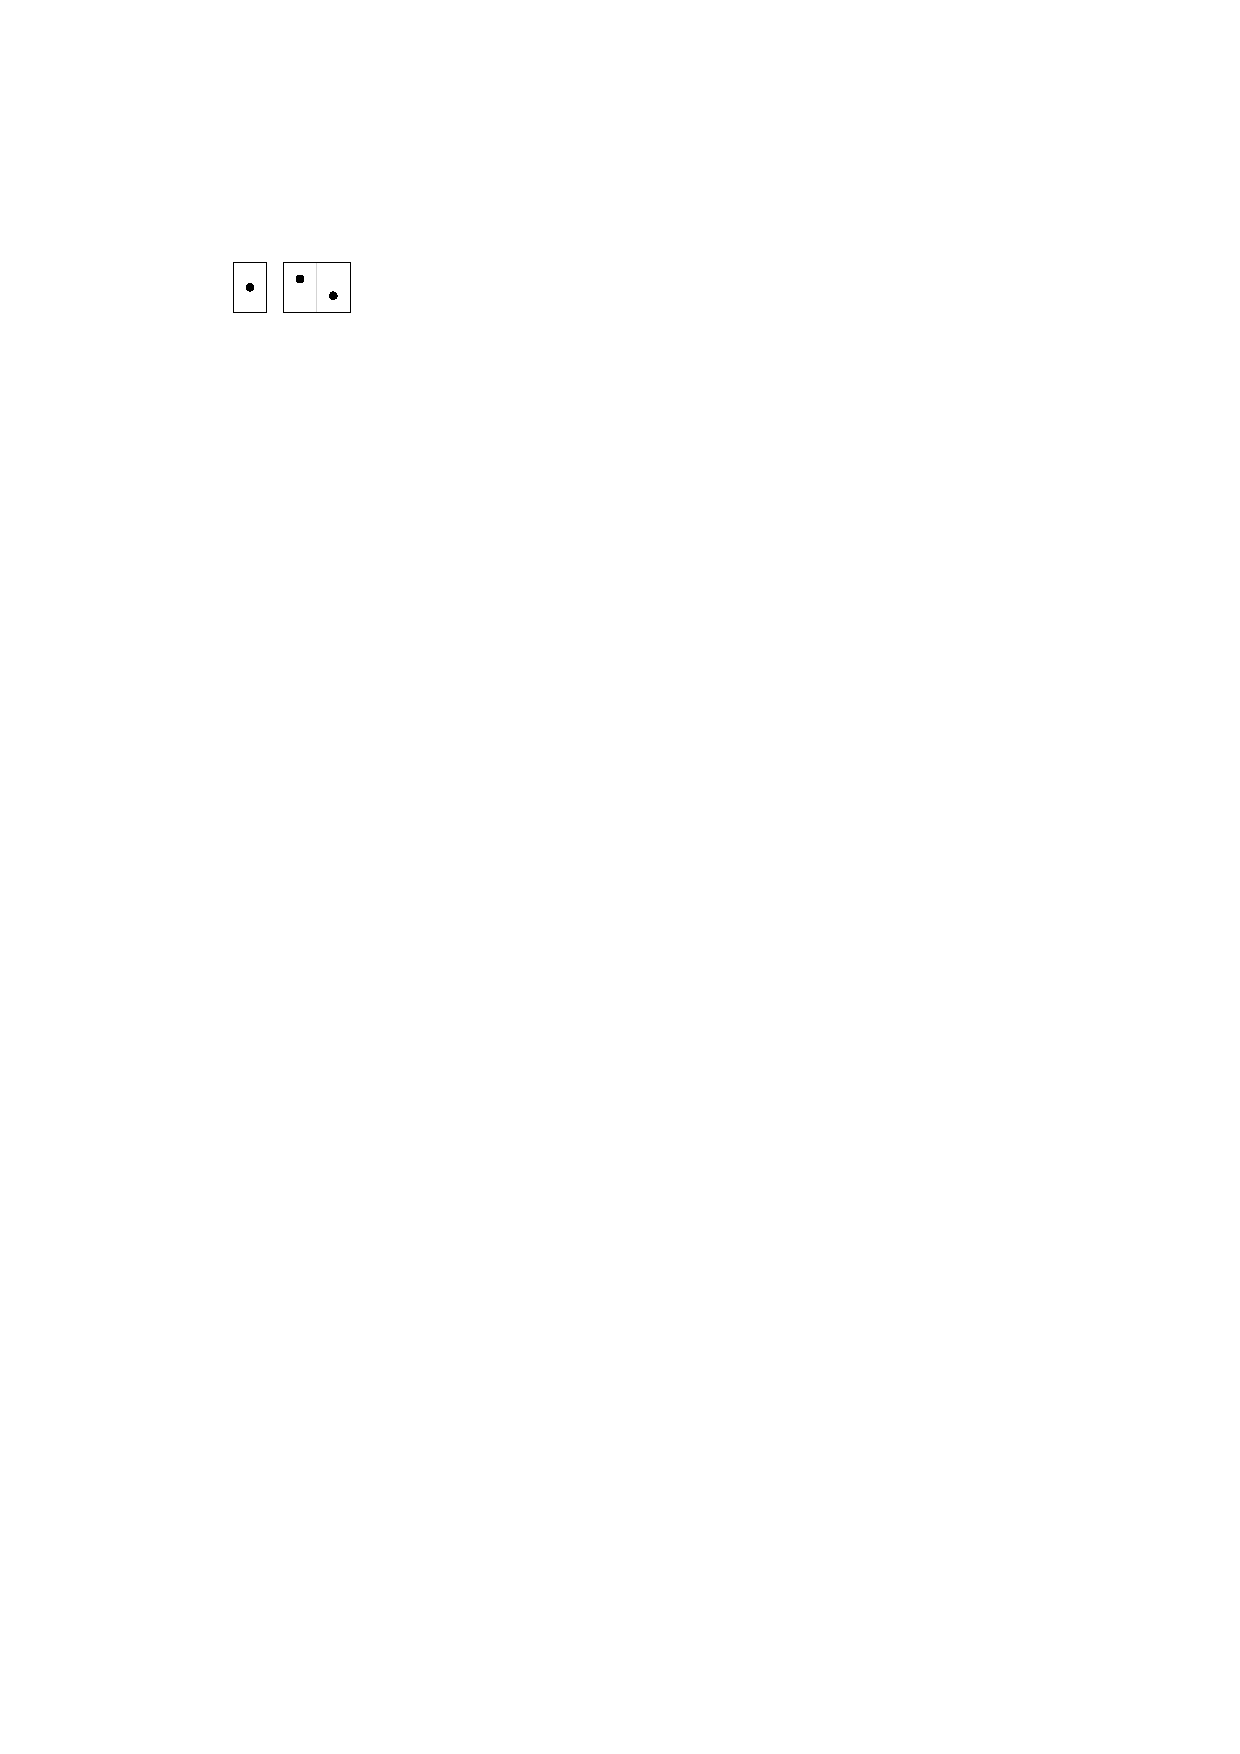
\includegraphics[scale=.625]{figs/cb} \\
     $c^3$ & $ac$ & $ca$ & $bc$ & $cb$ \\[.6cm]
  \end{tabular}

  \begin{tabular}{c@{\hspace{.6cm}}c@{\hspace{.6cm}}c@{\hspace{.6cm}}c@{\hspace{.6cm}}c@{\hspace{.6cm}}c}
     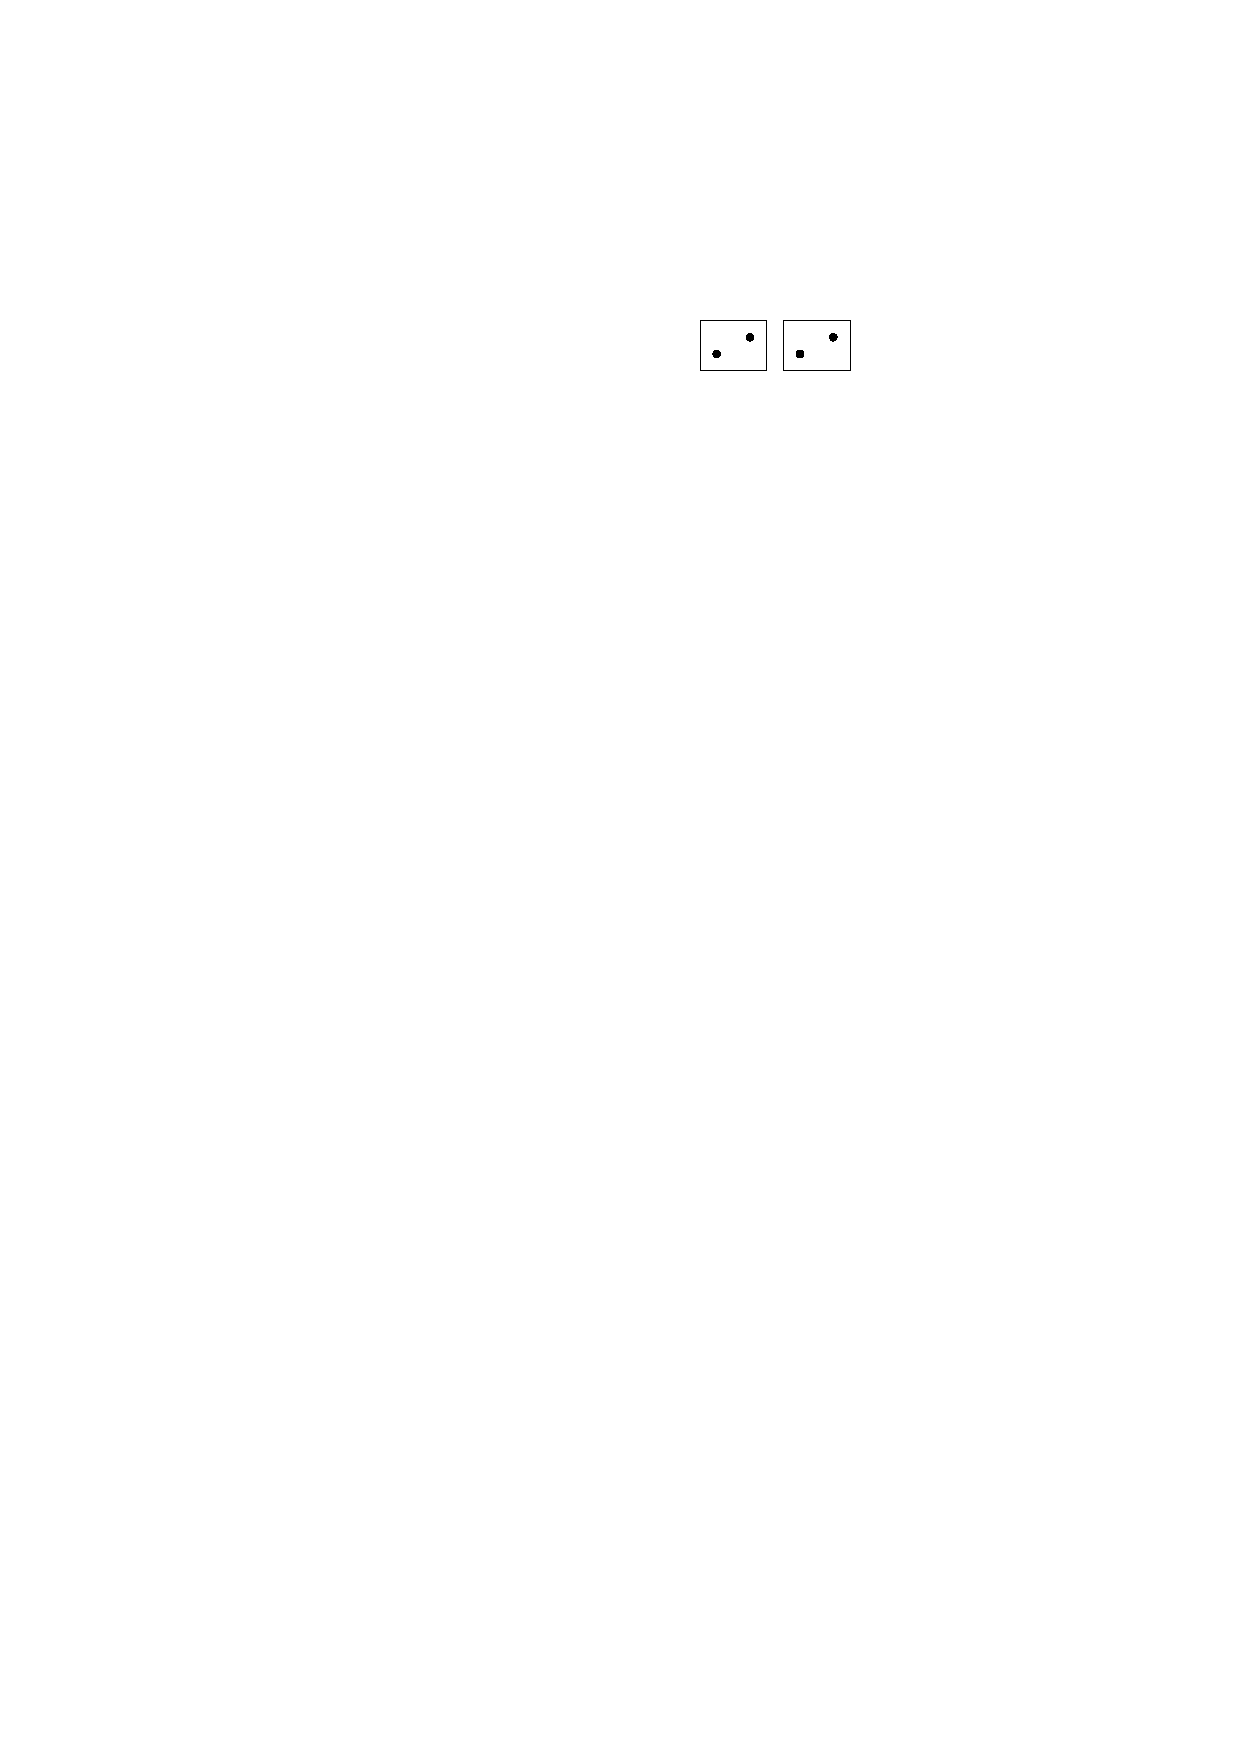
\includegraphics[scale=.625]{figs/a2} &
     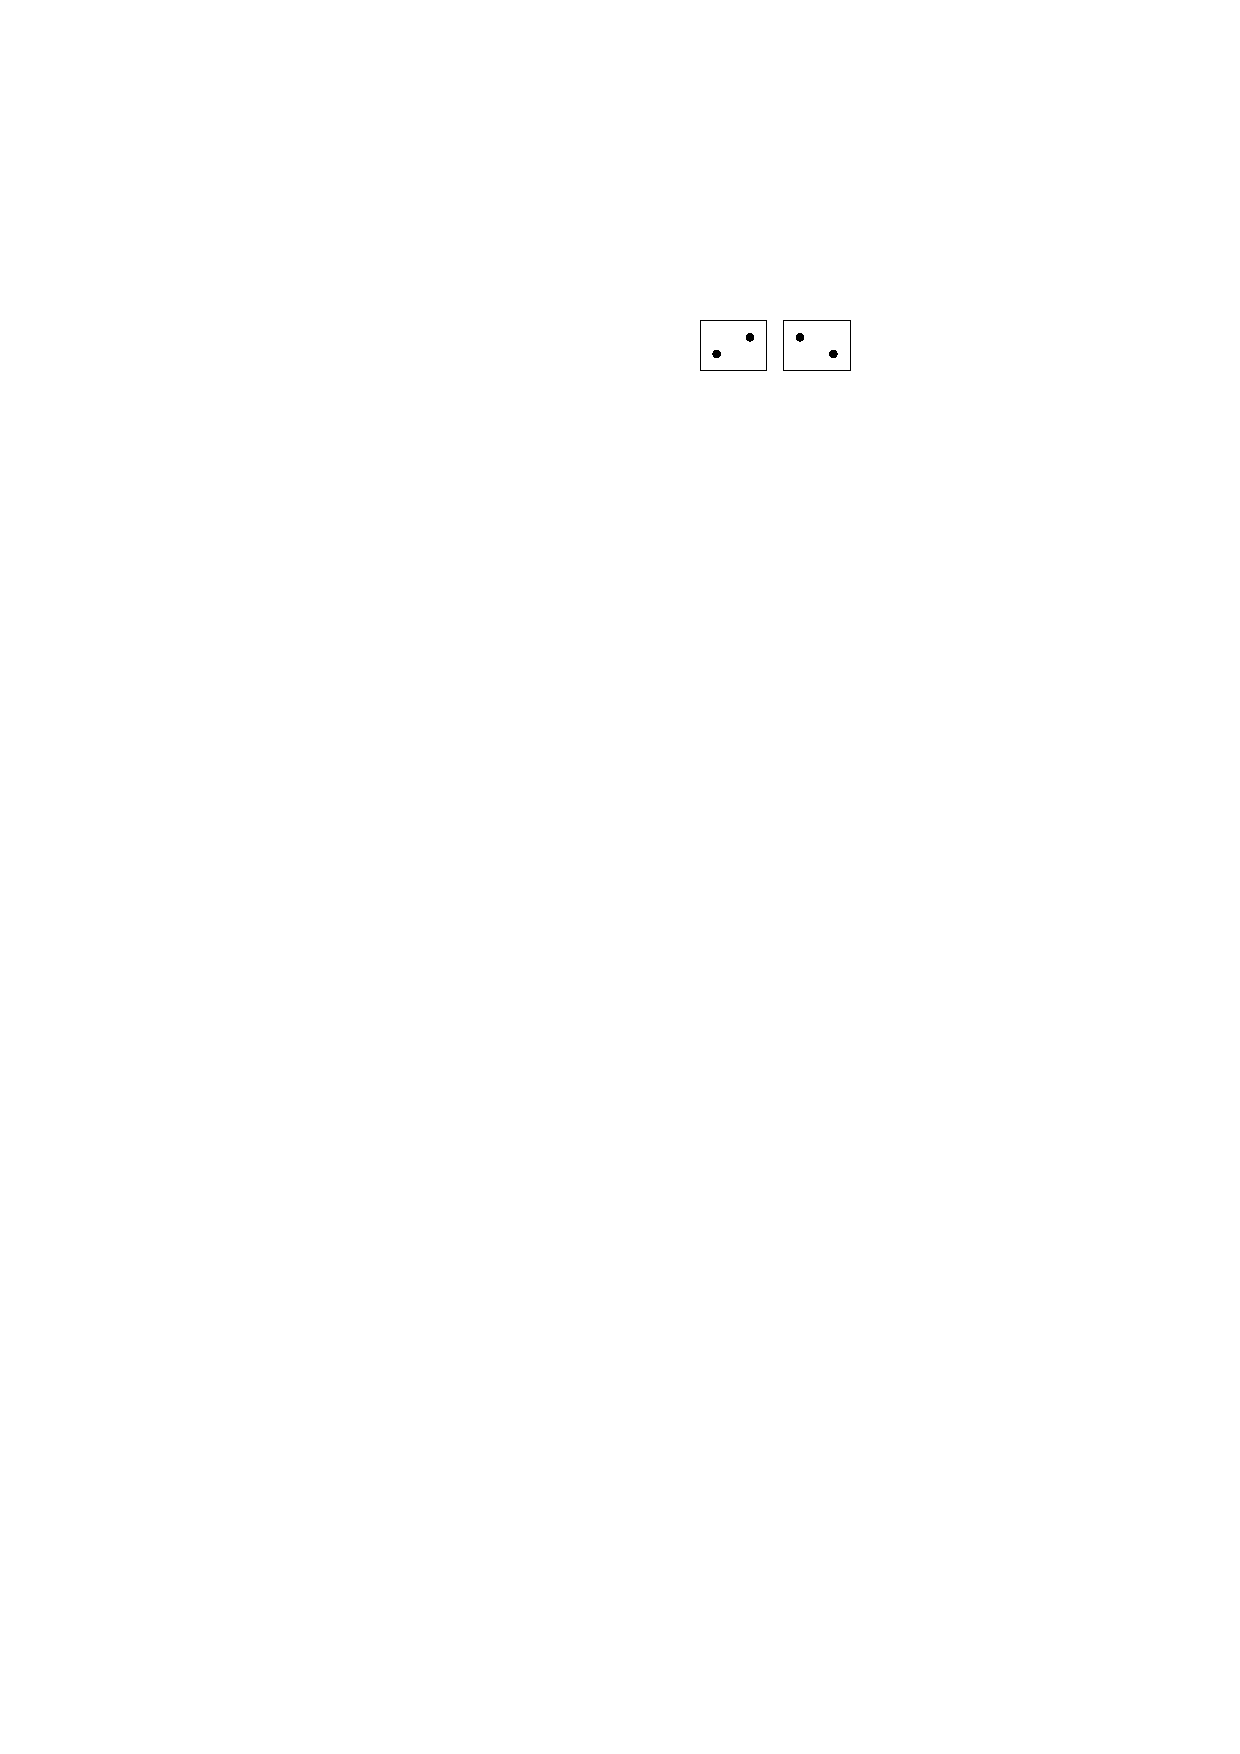
\includegraphics[scale=.625]{figs/ab} &
     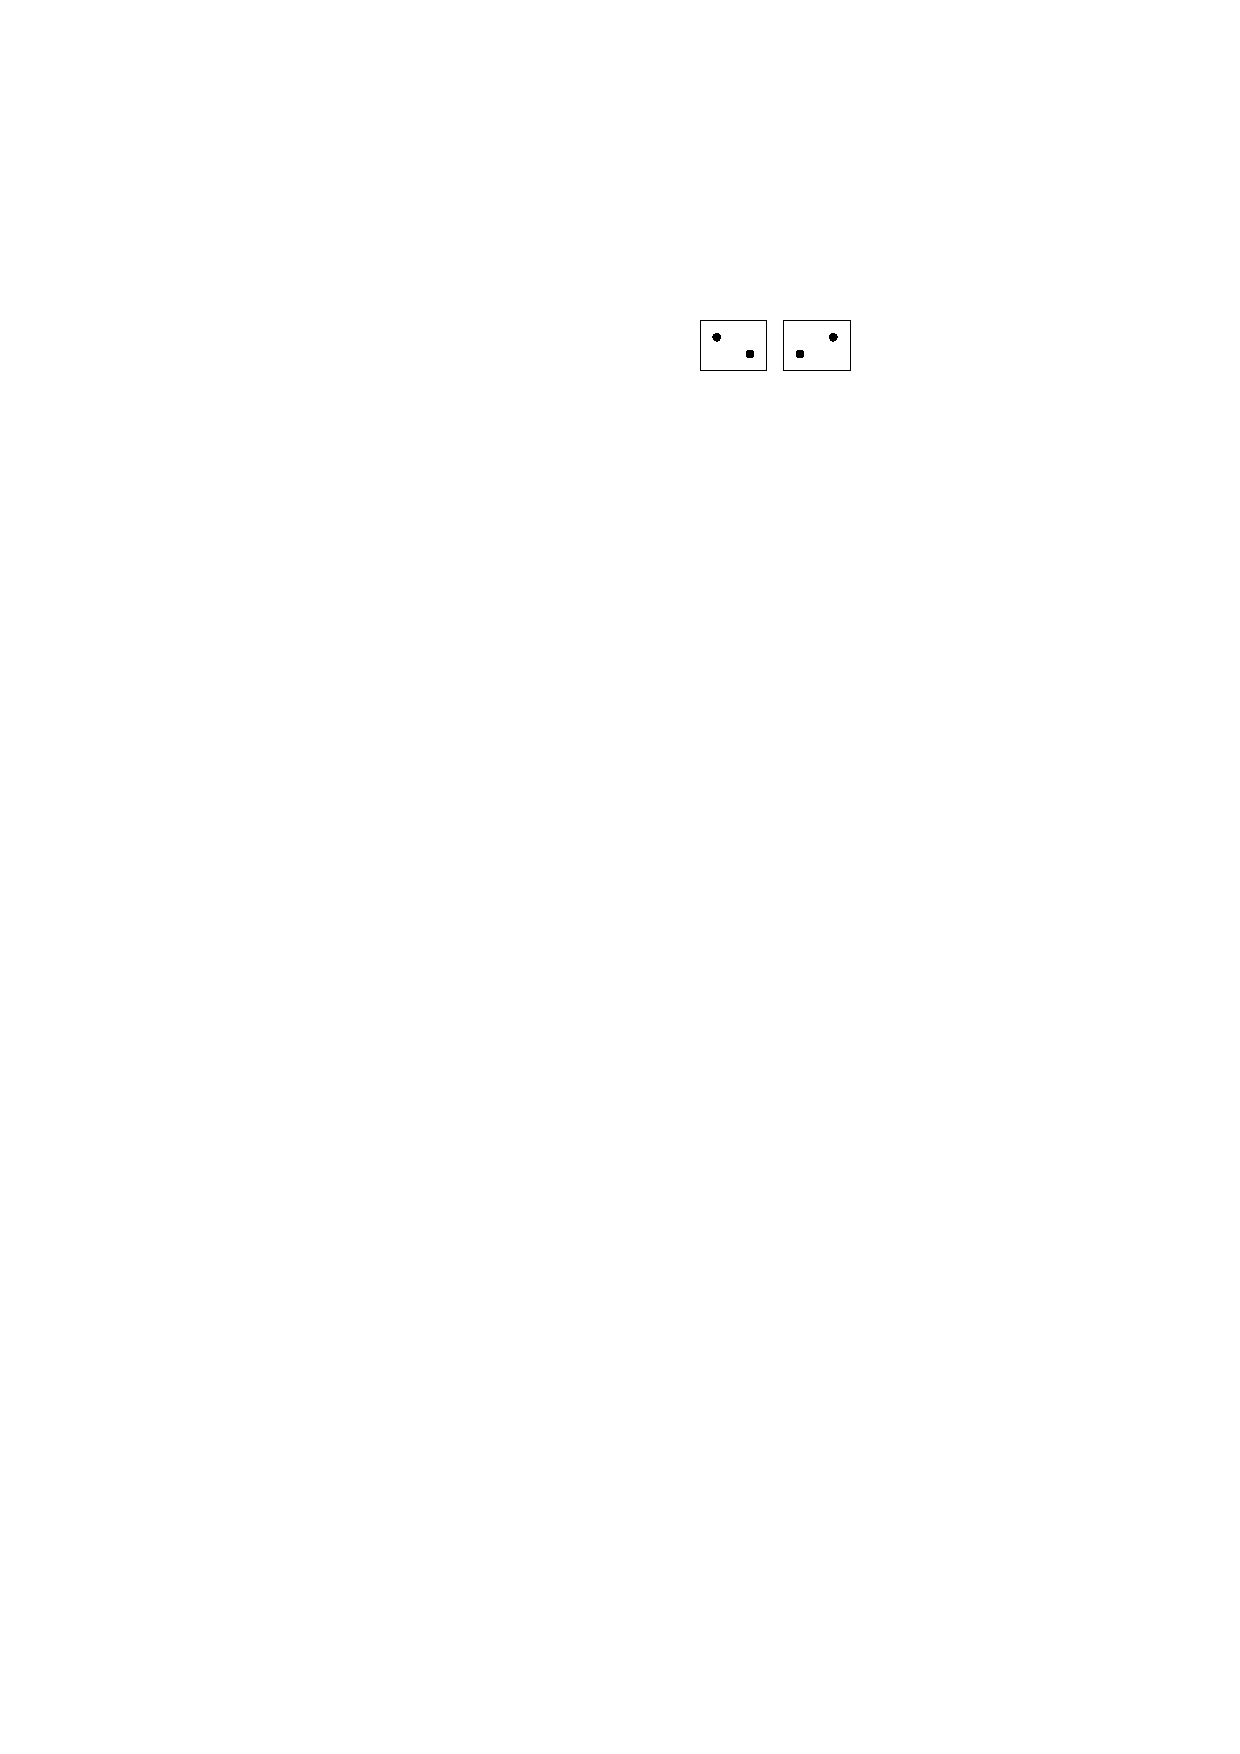
\includegraphics[scale=.625]{figs/ba} &
     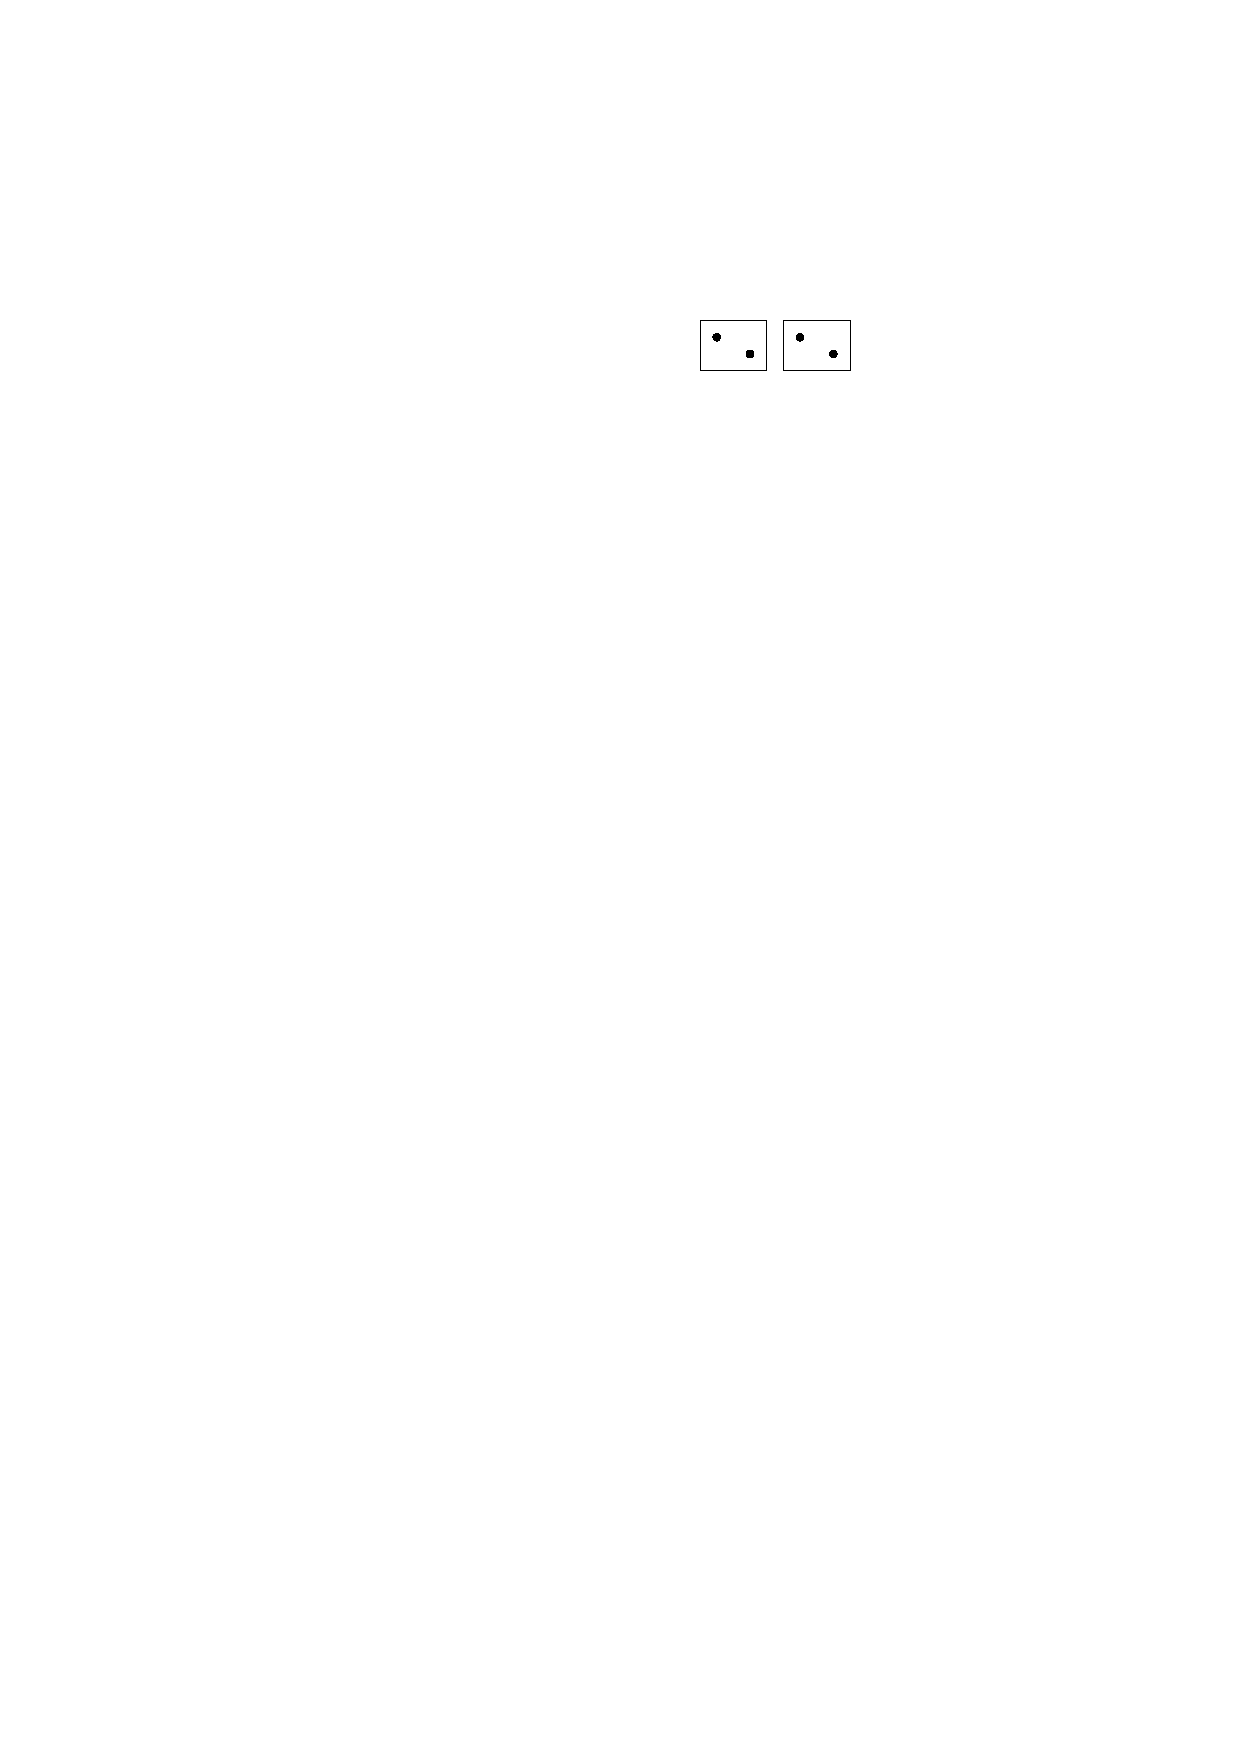
\includegraphics[scale=.625]{figs/b2} &
     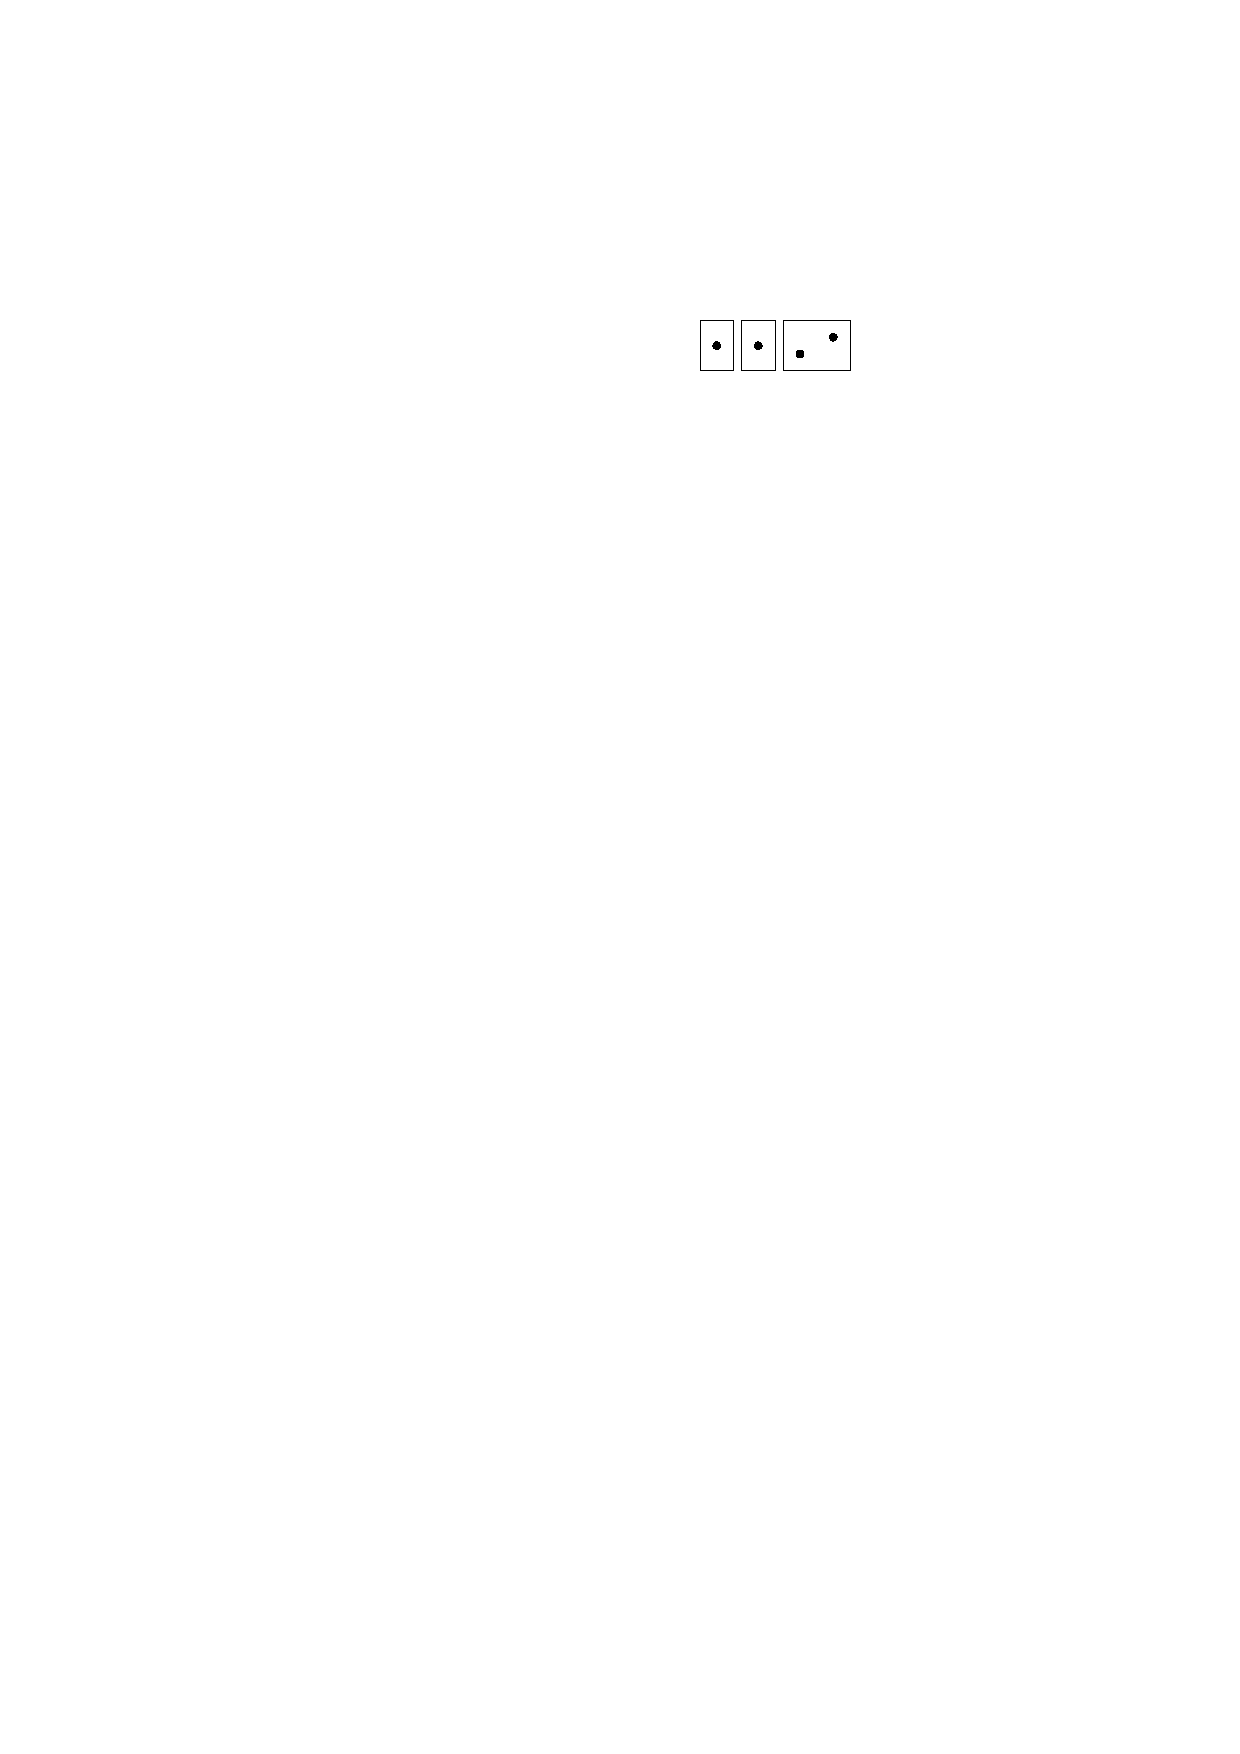
\includegraphics[scale=.625]{figs/c2a} &
     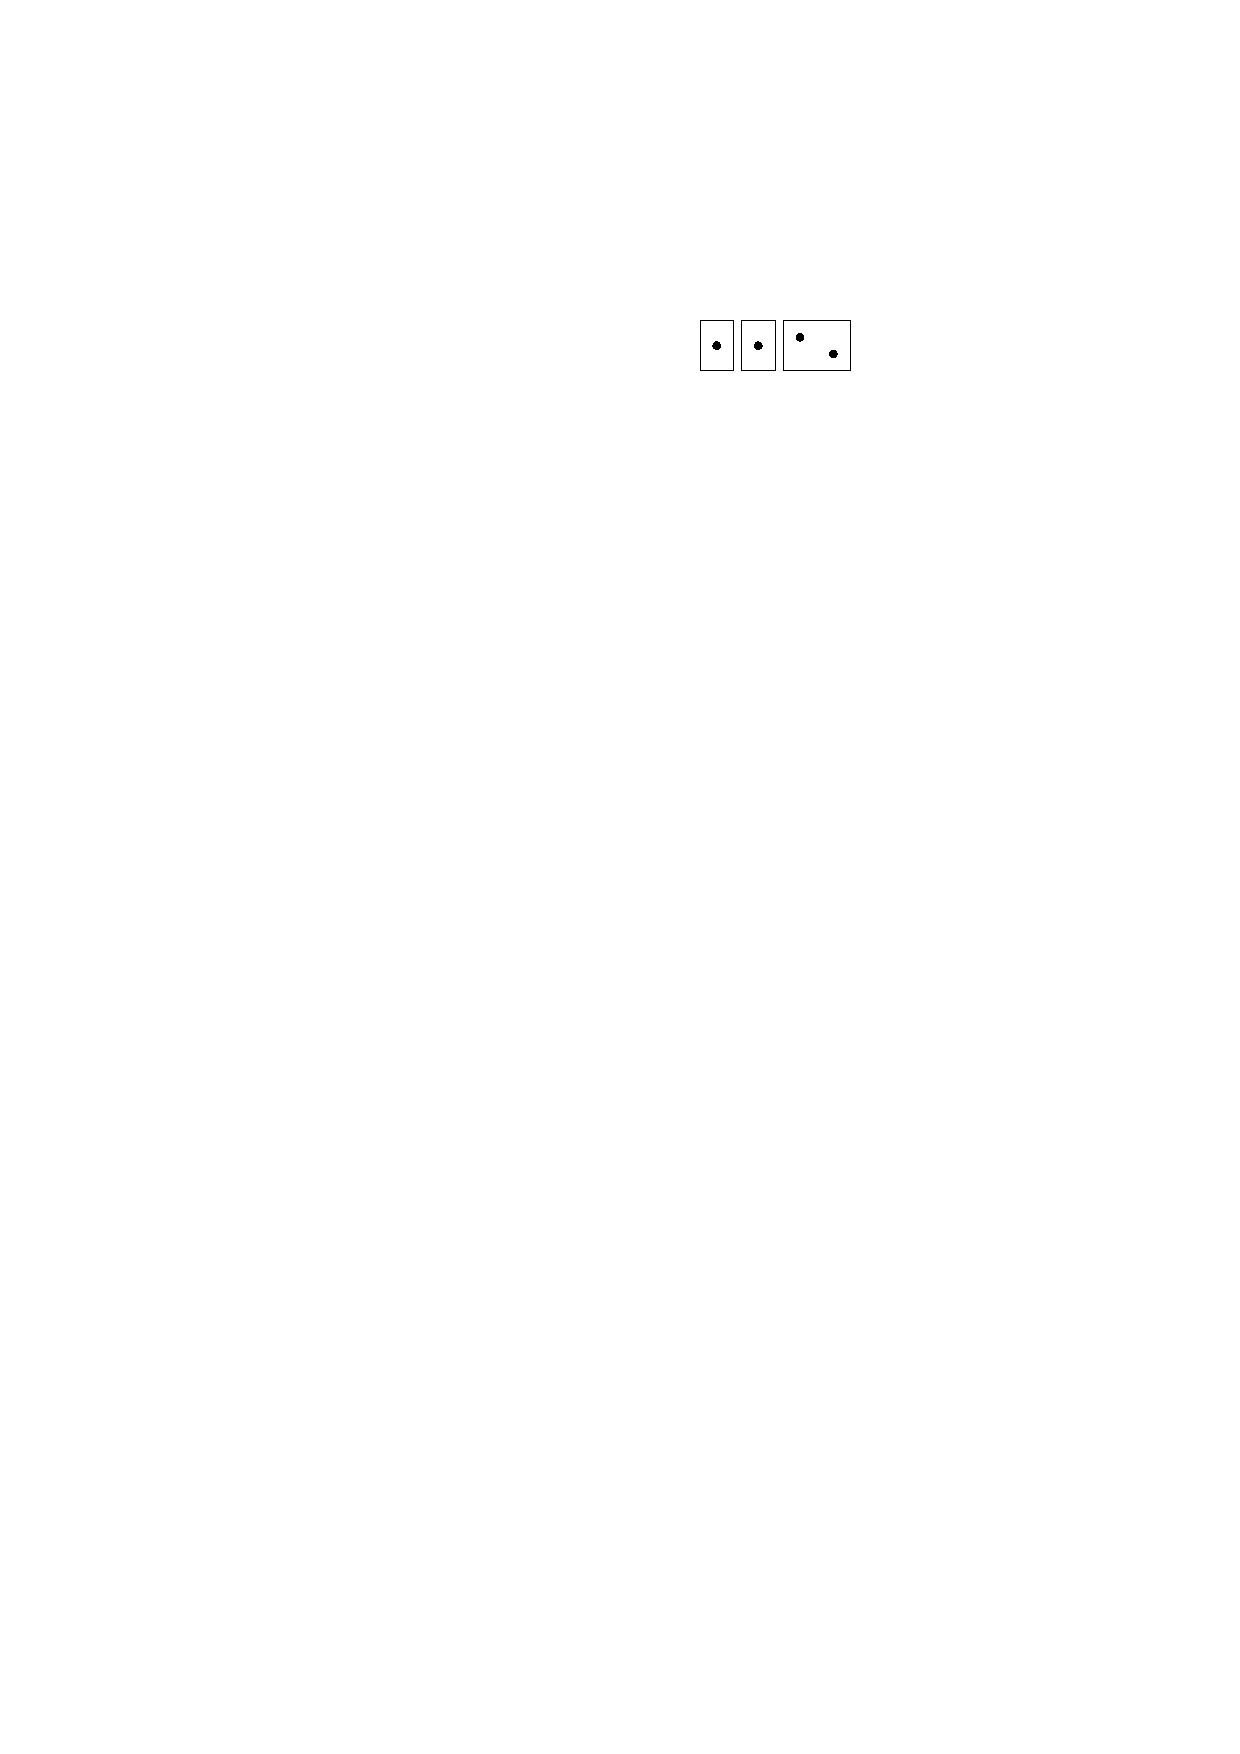
\includegraphics[scale=.625]{figs/c2b} \\
     $a^2$ & $ab$ & $ba$ & $b^2$ & $c^2a$ & $c^2b$ 
  \end{tabular}
  \end{center}
  \caption{The 11 types of groups}
  \figlabel{groups}
\end{figure}
We call these $a$-blocks, $b$-blocks, and $c$-blocks, respectively and
assume that the blocks of $B$ are iid and distributed so that 
each of these three block types occurs with probability
$a$, $b$, and $c=1-a-b$ respectively.   

These three types of blocks give rise to 11 types of groups, illustrated
in \figref{groups}. We name these groups by reading off the block types
that form the group from left to right so that, for example, a $ba$-group
is a $b$-block followed by an $a$-block.  This naming scheme is
convenient because the name of the group also gives the probability of
the group.

From this, we can deduce that
\[
    p_3 = c^3 + ac + ca + bc + cb
\]
and
\[
    p_4 = a^2 + ab + ba + b^2 + c^2a + c^2b \enspace .
\]

Each $ab$-, $ac$-, and $cb$-group always produces a block of size 1.
Each $ba$-group always produces a block of size 2.  A $c^3$-group produces
a block of size 1 with probability $2/3$ and produces a block of size
2 with probability $1/3$.

The remaining 6 group types may produce blocks of size 1 or of size
2 and the probability depends on the distribution of values within the
various block types.  For a $g$-group, we denote by $x_g$ the probability
that a group is a $g$-group and that it produces a block of size 1 so,
for example the probability that a group is an $a^2$-group and produces
block of size 2 is $a^2-x_{a^2}$.  With these notations, we can compute
$q_1$ and $q_2$:
\[
   q_1 = 2c^3/3 + ab + ac + cb + x_{ca} + x_{bc} + x_{a^2} + x_{b^2} + x_{c^2a} + x_{c^2b}
\]
\[
   q_2 = c^3/3 + ba + ca + bc + a^2 + b^2 + c^2a + c^2b
         - x_{ca} - x_{bc} - x_{a^2} - x_{b^2} - x_{c^2a} - x_{c^2b}
\]
%Unfortunately, all of this is still insufficient to prove an upper
%bound $\alpha < 1/2$. In particular, setting $a=1$ or $b=1$ and all
%other variables to 0, yields $q_1=p_3=0$, $q_2=p_4 = 1$, and $\alpha=1/2$.
%However, this is the only way to obtain a
%value of $\alpha = 1/2$.  
%In particular, if the product $ab$ is non-zero,
%then $\alpha$ is strictly less than $1/2$:
Define $x=x_{ca} + x_{bc} + x_{a^2} + x_{b^2} + x_{c^2a} + x_{c^2b}$.
The following upper bound on $\alpha$ is helpful:
\begin{align}
  \alpha & = \frac{q_1+2q_2}{3p_3 + 4p_4} \nonumber \\
%     & = \frac
%        {4c^3/3 + ab + ac + cb 
%         + 2ba + 2ca + 2bc + 2a^2 + 2b^2 + 2c^2a + 2c^2b
%         - x_{ca} - x_{bc} - x_{a^2} - x_{b^2} - x_{c^2a} - x_{c^2b}
%         }
%        {3c^3 + 6ac + 6bc + 8ab + 4a^2 + 4c^2b + 4a^2 + 4b^2 + 4c^2a} \\
     & = \frac
        { 4c^3/3 + 3ab + 3ac + 3bc + 2a^2 + 2b^2 + 2c^2a + 2c^2b - x}
        {3c^3 + 8ab + 6ac + 6bc + 4a^2 + 4b^2 + 4c^2a + 4c^2b} \eqlabel{clear} \\
     & = \frac{1}{2}- 
        \frac{c^3/6 + ab + x}
        {3c^3 + 8ab + 6ac + 6bc + 4a^2 + 4b^2 + 4c^2a + 4c^2b} \nonumber \\
     & = \frac{1}{2}- 
        \frac{c^3/6 + ab + x}{3q_3 + 4q_4} \nonumber \\
     & \le \frac{1}{2}- 
        \frac{c^3/6 + ab + x}{4q_3 + 4q_4} \nonumber \\
     & = \frac{1}{2}- 
        \frac{c^3/6 + ab + x}{4} \nonumber
\end{align}

Thus, we have a situation in which $\alpha$ can be very close $1/2$
if and only if $ab$, $c$, and $x$ are all very close to zero.  Since
$a+b+c=1$, this can only happen if one of $a$ or $b$ is close to one
and the remaining variables are close to zero.  Indeed, setting $a=1$
or $b=1$ and all other variables to 0, yields $q_1=p_3=0$, $q_2=p_4 =
1$, and $\alpha=1/2$.

To overcome this, we again study two consecutive rounds.  Recall that, by
definition, with probability $a^2-x_{a^2}$ a group is an $a^2$-group that
generates a block of size 2.  The key observation is that, by symmetry,
the resulting block is equally likely to an $a$-block or a $b$-block.
Similarly, with probability $b^2-x_{b^2}$ a group is a $b^2$-group
that generates a block of size 2 that is equally likely to be an
$a$-block or $b$-block.  Finally, with probability $c^3/3$, a group is
a $c^3$-group that generates a block of size 2 that is equally likely to
be an $a$-block or a $b$-block.  Letting $a'$, $b'$ and $c'=1-a'-b'=q_1$
denote the probabilities of $a$-, $b$-, and $c$-blocks in $R(B)$ we have
\[
   a',b' \ge (1/2)(a^2-x_{a^2}+b^2-x_{b^2}+c^3/3)\ge (1/2)(a^2+b^2+c^3/3-x)  \enspace .
\]  


Finally, let $q_1'$ and $q_2'$ denote the probabilities that a block
of $R(R(B))$ has size 1 and 2, respectively, and define 
\[
    \alpha' = \frac{q'_1+2q'_2}{3p_3 + 4p_4} \enspace .
\]
TODO: Fix this!
\begin{align}
    \alpha'(a,b,x) & = \frac{q'_1+2q'_2}{3p_3 + 4p_4} \\
            & \le \left(\frac{1}{2}-\frac{(c')^3/6+a'b'}{4}\right)
               \left(\frac{q_1+2q_2}{3p_3+4p_4} \right) \\
            & \le \left(\frac{1}{2}-\frac{q_1^3/6+(1/4)(a^2 + b^2 + c^3/3)^2}{4}\right)
               \left(\frac{q_1+2q_2}{3p_3+4p_4} \right) 
               \eqlabel{ap} 
\end{align}
This last expression is a function of 3 variables $a$, $b$ and $x$.
Maximizing this function over all $(a,b,x)\in[0,1]^3$ yields two global
maxima at $(\gamma,0,0)$ and $(0,\gamma,0)$ with $\gamma\approx0.547757022207$ and for which $\alpha(\gamma,0,0)=c_2$ with $c_2\approx 0.243739466166$. (The actual values of $\gamma$ and $\beta$ are each roots of degree 14 polynomials with integer coefficients---see the accompanying Sage worksheet.)

\begin{thm}
   For any $k\in\N$, $p_{k} \le c_2^{k/2} \le 0.49369977332^k$.
\end{thm}

\section{Remarks}

\bibliographystyle{plainurl}
\bibliography{franklin}

\end{document}


